\documentclass{beamer}
% \documentclass[handout]{beamer}

\mode<presentation> {%
	\usetheme[]{Boadilla}
	\usecolortheme{orchid}
	\setbeamercovered{transparent}
	\setbeamersize{text margin left=0.7cm}
  \setbeamersize{text margin right=0.7cm}
  \setbeamertemplate{enumerate item}[square]
  \setbeamertemplate{enumerate subitem}[circle]
  \setbeamertemplate{enumerate subsubitem}[>]
  \setbeamertemplate{itemize item}[square]
  \setbeamertemplate{itemize subitem}[circle]
  \setbeamertemplate{itemize subsubitem}[>]

  
\usepackage{bm}
\usepackage[utf8]{inputenc}
\usepackage[spanish]{babel}
\usepackage[normalem]{ulem}
\usepackage{times}
\usepackage[T1]{fontenc}
\usepackage{graphicx}
\usepackage{multirow}
\usepackage{pifont}
\usepackage{rotating}
\usepackage{colortbl}
\usepackage{amssymb}

\usepackage[framed]{mcode}
\usepackage{verbatim}
\lstset{literate={ñ}{{\~n}}1}

\definecolor{olivegreen}{rgb}{0.0,0.5,0.0}
\definecolor{general}{rgb}{0.9 0.9 1}%
% \newrgbcolor{colorsistema}{0 1 1}
% \newrgbcolor{colorviolet}{0.9 0.8 1}

\title[Procesamiento de Señales]{Señales Aleatorias}
\author[Jesús Chacón Sombría] {%
 	\textit{Ingeniería Electrónica de Comunicaciones}\\
 	\vspace{0.6cm}%
	\small Jesús Chacón Sombría%
}%

\institute[DACYA. UCM] {%\inst{1}%
	\footnotesize  Departamento de Arquitectura de Computadores y Automática\\
  Universidad Complutense de Madrid
}

\date[Señales Aleatorias] % (optional)
{\footnotesize Curso 2021-2022}%{\today / Master}
\subject{Talks}

\pgfdeclareimage[height=0.75cm]{logo}{ucm}

\usepackage[absolute,overlay]{textpos}
\setlength{\TPHorizModule}{1mm}
\setlength{\TPVertModule}{1mm}
\newcommand{\MyLogo}{%
\begin{textblock}{14}(116.0,0.6)
  \pgfuseimage{logo}
\end{textblock}
}

\makeatletter
\numberwithin{section}{part}
\AtBeginPart{
\beamer@tocsectionnumber=0\relax
\frame{\partpage}
}
\makeatother

\begin{document}

\begin{frame}
  \titlepage
\end{frame}

\newcommand*\oldmacro{}%
\let\oldmacro\insertshorttitle%
\renewcommand*\insertshorttitle{%
	%\MyLogo
\oldmacro\hfill%
}

\AtBeginSection[]
{
  \begin{frame}%<beamer>
    \frametitle{Esquema}
  \small
    \tableofcontents[sectionstyle=show/shaded,subsectionstyle=show/shaded/hide]
  \end{frame}
}

\AtBeginSubsection[]
{
  \begin{frame}%<beamer>
    \frametitle{Esquema}
  \small
   \tableofcontents[sectionstyle=show/shaded,subsectionstyle=show/shaded/hide]
      \end{frame}
}

  

%%%%%%%%%%%%%%Empieza la presentacion%%%%%%%%%%%%%%%%%%%%%%%%%%%%%%%%%%%%

%\begin{frame}
%\frametitle{Esquema}
 %   \tableofcontents
%\end{frame}

\section{Objetivos}

\begin{frame}
\frametitle{Objetivos del tema}

\begin{itemize}
\item Aprender a distinguir desde un punto de vista matemático el comportamiento de las señales deterministas y los diferentes tipos de señales aleatorias (estacionarias, ergódicas, proceso de Markov).

\visible<2->{
\item Definir matemáticamente las propiedades más relevantes de:
}
\begin{itemize}
\normalsize
\visible<3->{
\item Variables aleatoria: distribución/densidad de probabilidad, valor medio, valor cuadrático medio, varianza, correlación
}


\visible<4->{
\item Señales aleatorias: valor medio, valor cuadrático medio, covarianza, autocorrelación y correlación cruzada, densidad espectral de potencia
}



\end{itemize}

\visible<5->{\item Procesamiento de señales aleatorias a través de las técnicas de procesamiento de señales deterministas}

\end{itemize}

\end{frame}


 %%%%%%%%%%%%%%Empieza la presentacion%%%%%%%%%%%%%%%%%%%%%%%%%%%%%%%%%%%%

%\begin{frame}
%\frametitle{Esquema}
 %   \tableofcontents
%\end{frame}

\section{Introducción}


\begin{frame}\frametitle{Señales deterministas y estocásticas I}
    \footnotesize
    \begin{itemize}
        \item \alert{Señales deterministas}: 
        \begin{itemize}\footnotesize
            \item Toman siempre el mismo valor para el mismo instante de tiempo. 
            \item Se representan por una única secuencia continua/discreta de valores. 
            \item El valor en cada instante puede ser definido de forma explícita.
            \item Función matemática determinista:  $t \rightarrow f(t)$\\\scriptsize\color{gray} \emph{relaciona el valor de la señal con el valor de variable independiente (tiempo).}
        \end{itemize}
        \item \alert{Señales estocásticas/aleatorias}: 
        \begin{itemize}\footnotesize
            \item No toman siempre el mismo valor para un mismo instante de tiempo. 
            \item Colección infinita de secuencias continuas/discretas de valores. 
            \item El valor en cada instante es una variable aleatoria.
            \item El comportamiento se define a través de una función de probabilidad.
        \end{itemize}
    \end{itemize}
\end{frame}

%%%%%%%%%%%%%%%%%%%%%%%%%%%%%%%%%%%%%%%%%%%%%%%%

\begin{frame}\frametitle{Señales deterministas y estocásticas II}
    \begin{columns}[T]
        \begin{column}{6cm}
            \small
            \centering Señal determinista:\\
            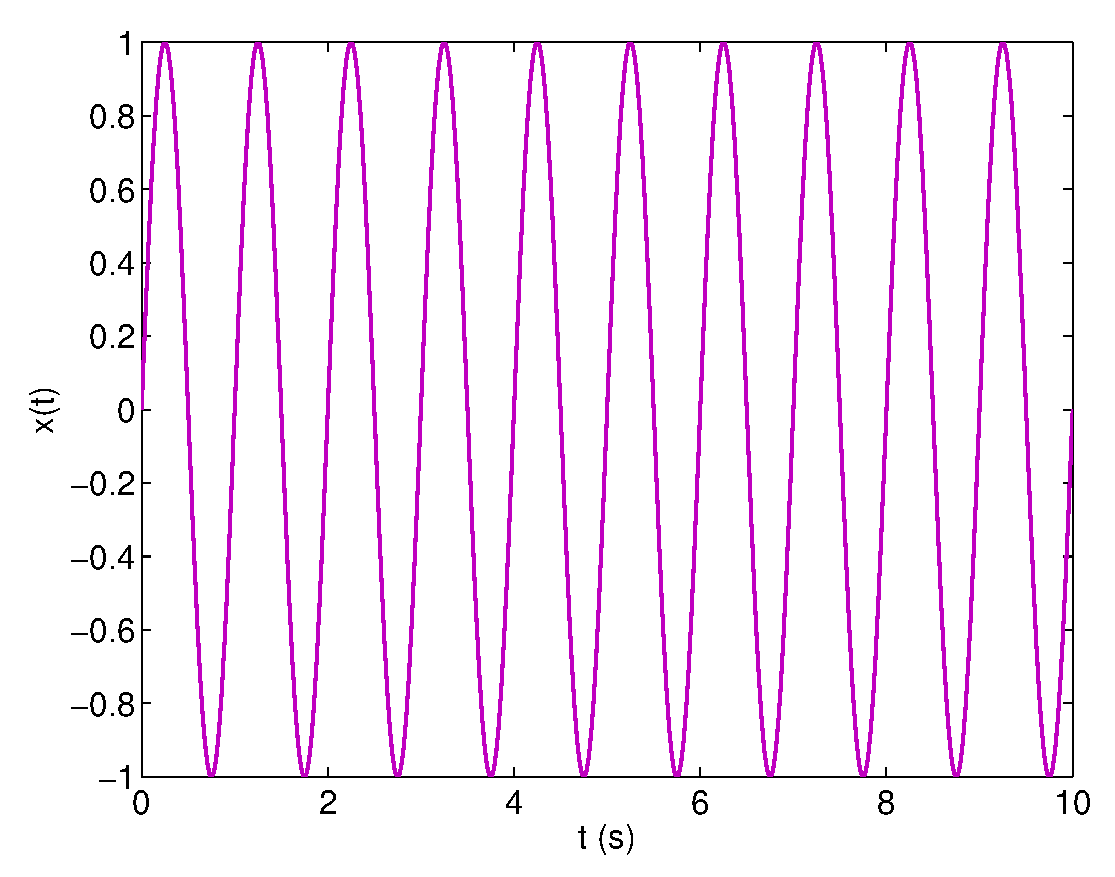
\includegraphics[width=6cm]{./Figures/SignalDeterministic.eps} 
            $x(t)=sen(\omega t)$
        \end{column}
        \begin{column}{6cm}
            \small
            \centering Señal estocástica:\\
            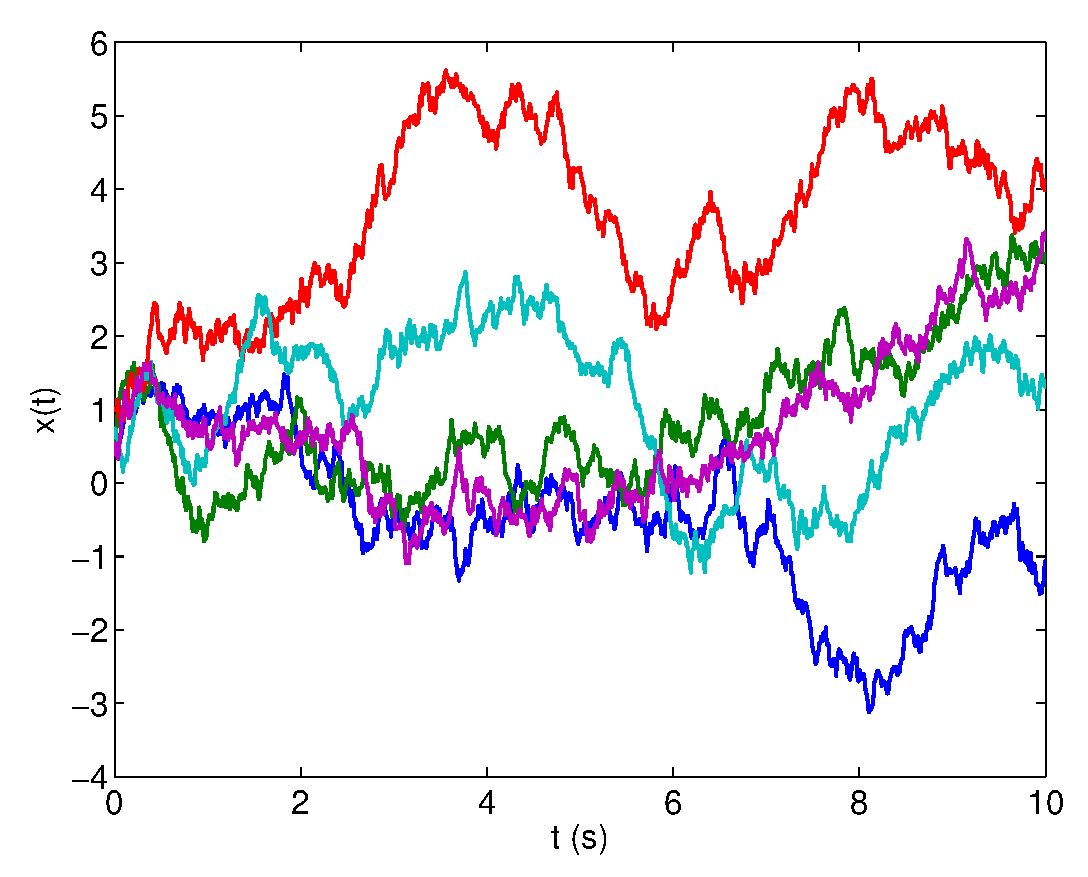
\includegraphics[width=6cm]{./Figures/SignalRandom.eps}\\
            $p(x(t_0),x(t_1),x(t_2),\dots,x(t_\infty))$
        \end{column}
    \end{columns}
\end{frame}

%%%%%%%%%%%%%%%%%%%%%%%%%%%%%%%%%%%%%%%%%%%%%%%


\begin{frame}\frametitle{Señales deterministas y estocásticas III}
    \begin{itemize}
        \item ¿Las señales reales son deterministas o estocásticas?
        \vspace{0.1cm}
        \begin{itemize}\footnotesize
            \item \alert{Argumento 1:} No existen señales totalmente deterministas.
            \begin{itemize}\scriptsize
                \item Puede existir algún fenómeno que no haya sido tenido en cuenta.
                \item Los valores de la señal no están totalmente determinados a priori.
            \end{itemize}
            \item \alert{Argumento 2:} Todas las señales son intrínsecamente deterministas.
            \begin{itemize}\scriptsize
                \item Desconocimiento parcial del proceso que las genera. 
                \item Por tanto no son realmente aleatorias.
            \end{itemize}
        \end{itemize}
        \vspace{0.1cm}
        \item Clasificación \alert{determinista} vs. \alert{estocástica}:
        \vspace{0.1cm}
        \begin{itemize}\footnotesize
            \item Atiende al tratamiento que se le desea dar a la señal,
            \vspace{0.1cm}
            \item No a la forma en que la señal ha sido generada.
        \end{itemize}
    \end{itemize}
\end{frame}
\section{Variables aleatorias}
 %%%%%%%%%%%%%%Empieza la presentacion%%%%%%%%%%%%%%%%%%%%%%%%%%%%%%%%%%%%

%\begin{frame}
%\frametitle{Esquema}
 %   \tableofcontents
%\end{frame}

\subsection{Una variable aleatoria}

\begin{frame}\frametitle{Definición de una variable aleatoria}
  \begin{itemize}
    \item \alert{Variable aleatoria$^1$ $X$ (continua o discreta)}:
    \begin{itemize}
      \item Representa el resultado de un experimento aleatorio.
      \item Su valor no es conocido a priori.
      \item ¿Cómo podemos caracterizarla?
      \begin{itemize}
        \item ¿Que valores puede tomar?
        \item ¿Es igual de probable cada valor?
      \end{itemize}
    \end{itemize}
  \end{itemize}

  \begin{columns}[T]
    \begin{column}{5cm}
      \scriptsize
      \centering \color{olivegreen} Ejemplo discreto: X valores de un dado
      \color{gray}$p_X(x)=\frac{1}{6}$

      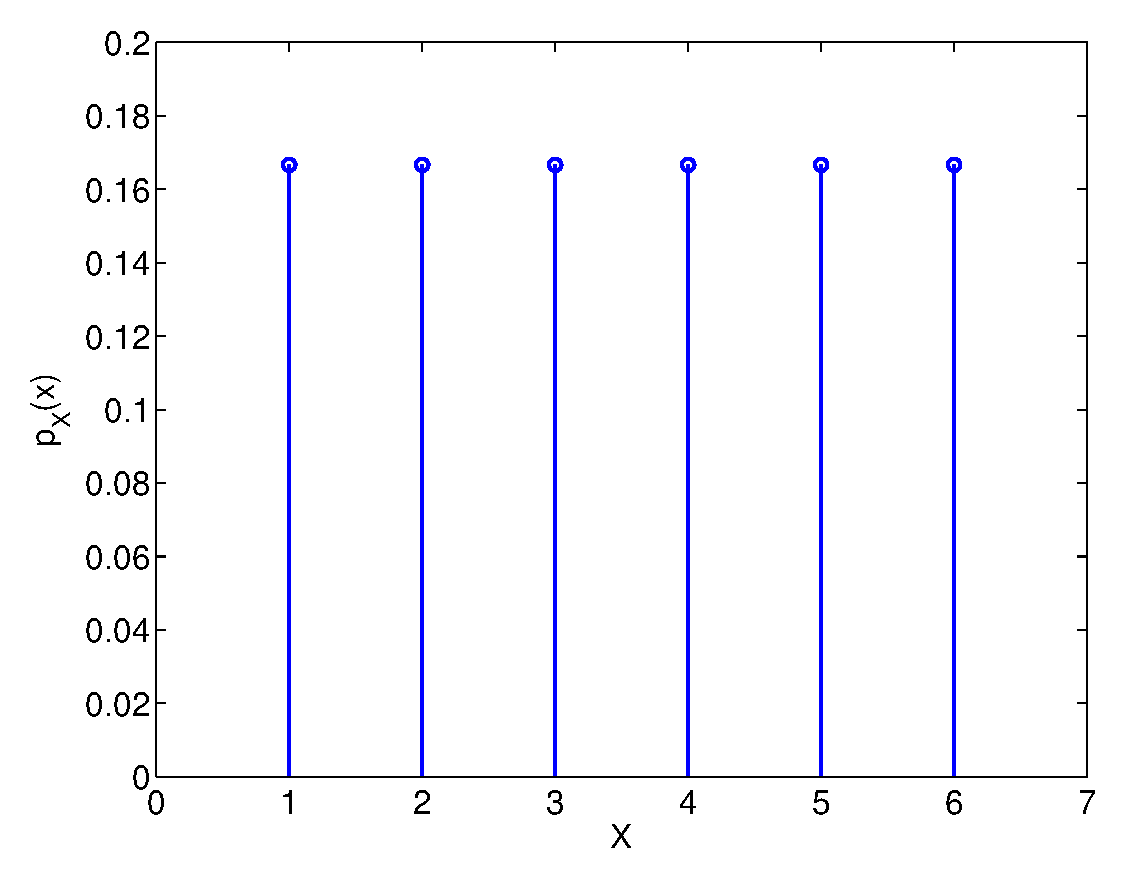
\includegraphics[width=3cm]{./Figures/ProbDiscreta.eps}
    \end{column}
    \begin{column}{6cm}\centering
      \scriptsize

      \centering \color{olivegreen} Ejemplo continuo: X tiempo de espera

      \color{gray}$p_X(x)=\mathcal{U}_{X\in[0,30]}(x)$

      \vspace{0.2cm}
      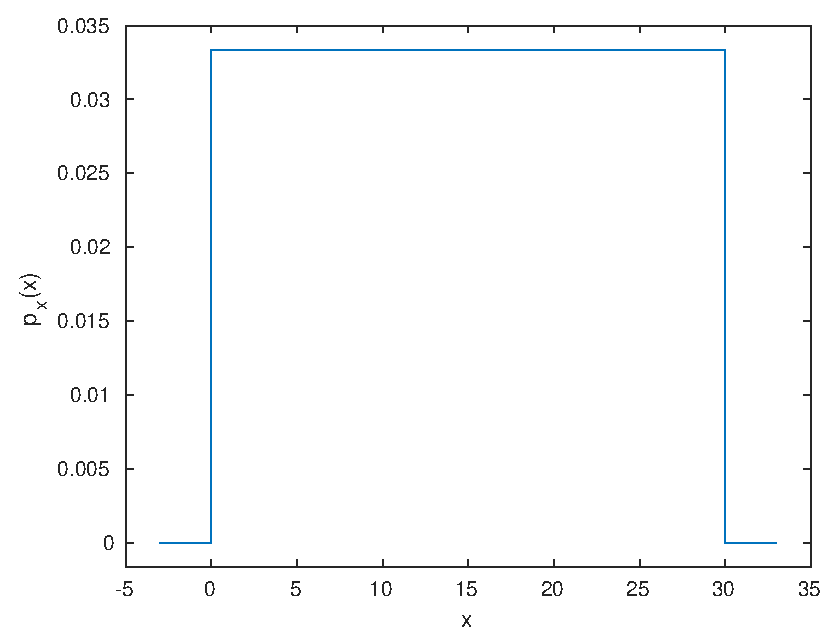
\includegraphics[height=2cm]{./Figures/ProbContinua.eps}
      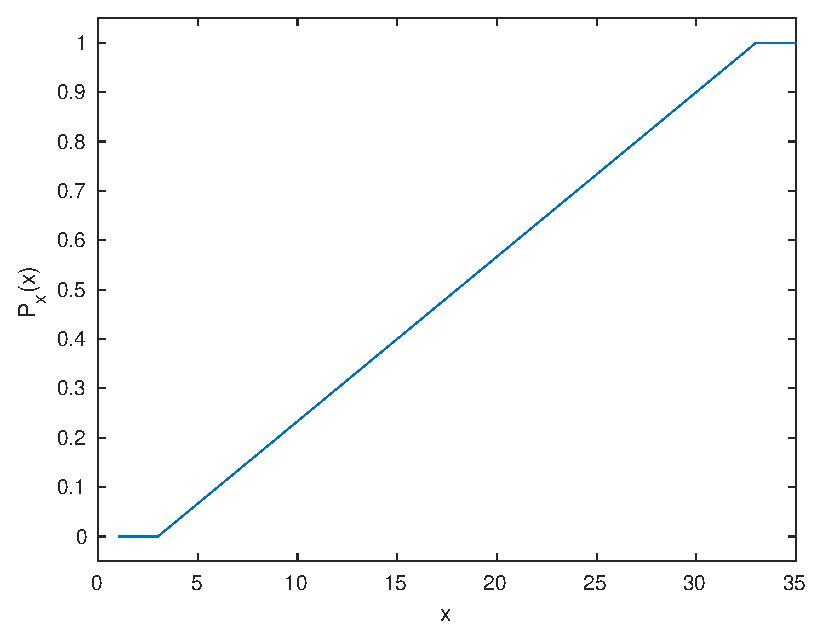
\includegraphics[height=2cm]{./Figures/ProbDistContinua.eps}
    \end{column}
  \end{columns}


  \rule{10cm}{0.04ex}

  \scriptsize
  $^1$En estadística es habitual definir la variable aleatoria con mayúsculas y sus valores con minúsculas.
\end{frame}



\begin{frame}\frametitle{Definición de una variable aleatoria}
  \begin{itemize}
    \item \alert{Para variables discretas:}
    \vspace{0.1cm}
    \begin{itemize}\footnotesize
      \item Función de \color{olivegreen}\emph{masa de probabilidad}: \color{blue}$p_X(x_i)=Probabilidad(X=x_i)$\color{black}
      \vspace{0.1cm}
      \item Propiedades:
      \begin{itemize}
        \item $0\le p_X(x_i)\le 1$
        \vspace{0.1cm}
        \item $\sum_{x\in X} p_X(x)=1$
      \end{itemize}
    \end{itemize}
    \vspace{0.2cm}
    \item \alert{Para variables continuas:}
    \vspace{0.1cm}
    \begin{itemize}\footnotesize
      \item \color{olivegreen}\emph{Distribución de probabilidad}: \color{blue}$P_X(x)=Probabilidad(X\le x)$\color{black}
      \vspace{0.1cm}
      \item \color{olivegreen}\emph{Densidad de probabilidad}: \color{blue}$p_X(x)=\frac{\partial P_X(x)}{\partial x}$\color{black}
      \vspace{0.1cm}
      \item Propiedades:
      \begin{itemize}
        \item $p_X(x)\ge 0$ $\rightarrow P_X(x)$ es una función creciente
        \vspace{0.1cm}
        \item $P_X(x)=\int_{-\infty}^x p_X(y)dy \rightarrow P_X(\infty)=1$
      \end{itemize}
    \end{itemize}
  \end{itemize}



  % \rule{10cm}{0.04ex}

  % \scriptsize
  % $^1$En estadística es habitual definir la variable aleatoria con mayúsculas y sus valores con minúsculas.
\end{frame}

%%%%%%%%%%%%%%


\begin{frame}\frametitle{Estadísticos}
  % \begin{itemize}
  %   \item ¿Qué más podemos decir sobre la variable aleatoria?
    \begin{itemize}
      \item Un \alert{estadístico} es una medida cuantitiva de una muestra.
      \begin{itemize}
        \item Valor esperado de alguna función $g(x)$.
        \begin{itemize}
          \vspace{0.1cm}
          \item \alert{Continuo:} \hspace{0.1cm}\\\vspace{0.1cm}$E(g(X))=\int_{-\infty}^{\infty}g(x) p_X(x)dx$
          \vspace{0.1cm}
          \item \alert{Discreto:}\\\vspace{0.1cm}$E(g(X))=\sum_{x_i \in X} g(x_i)p_X(x_i)$
        \end{itemize}
      \item Respecto a la probabilidad $p_X(x)$.
      \end{itemize}
      \item Trata de inferir o estimar una propiedad de la población.
    \end{itemize}
    \footnotesize
        % \item Estadísticos frecuentes:
    % \begin{itemize}
    %   \item $\mu_x=E\{X\}$ (media)
    %   \item $\sigma_x^2=E\{(X-\mu_x)^2\}$ (varianza)
    %   \item $E\{X^2\}=\sigma_x^2+\mu_x^2$ (valor cuadrático medio)
    % \end{itemize}
  % \end{itemize}
\end{frame}
  

\begin{frame}\frametitle{Estadísticos de una variable aleatoria}
  \footnotesize

% \vspace{-0.2cm}
  \begin{itemize}
    \item Estadísticos/características habituales (expresiones continuas$^1$)

    \begin{itemize}\footnotesize
      \item \alert{Valor medio}:\\\vspace{0.1cm}$\mu_X \triangleq E(X)$ $=\int_{-\infty}^{\infty}x p_X(x)dx$
      \item \alert{Valor cuadrático medio:}\\\vspace{0.1cm}$E(X^2)$ $=\int_{-\infty}^{\infty}x^2 p_X(x)dx$
      \item \alert{Varianza$^2$:}\\\vspace{0.1cm}$\sigma^2_X \triangleq E((X-\mu_x)(X-\mu_x))=\int_{-\infty}^{\infty}(x-\mu_x)(x-\mu_x) p_X(x)dx$ $=E(X^2)-\mu_x^2$
    \end{itemize}

  \end{itemize}

% \vspace{-0.3cm}

  \rule{11cm}{0.04ex}
  \scriptsize
  $^1$La relación discreta se puede sacar de la continua, construyendo una función densidad de probabilidad para la variable aleatoria discreta:  $p_{X_C}(x)=\sum_{x_i \in X} p_X(x_i)\delta(x-x_i) \rightarrow$
  $E(g(X_C))\!=\!\int_{-\infty}^{\infty}\!g(x)\! \sum_{x_i \in X} p_X(x_i)\delta(x\!-\!x_i)dx\!=\!\sum_{x_i \in X} g(x_i)p_X(x_i)=E(g(X))$. Equivale a sustituir las integrales por sumarios en las relaciones de las variables continuas. Por lo tanto, podemos definir únicamente las relaciones continuas y extrapolar las discretas.

  \vspace{0.2cm}

  $^2$Relación entre $\sigma^2_X$, $\mu_X$ y $E(X^2)$:  $\sigma^2_X\!=\!\! \int_{-\infty}^{\infty}\!\!(x^2\!-\!2 \mu_X x\!+\! \mu_X^2) p_X(x)dx=$ $=E(X^2)-2\mu_X \int_{-\infty}^{\infty}x p_X(x)dx+ \mu_X^2  \int_{-\infty}^{\infty}p_X(x)dx=E(X^2)-2\mu_X^2+\mu_X^2 $

\end{frame}

%%%%%%%%%%%%%%%%%%%%%%%%%%%%%%%%%%%%%%%%%%%%%%%%%


\begin{frame}\frametitle{Variables aleatorias comunes}
  \begin{itemize}
    \item \alert{Distribución uniforme}:\hspace{0.2cm}
    \small$p_X(x)=\mathcal{U}_{X \in [a,b]}(x)=\left \{\begin{array}{cl}\frac{1}{b-a}  &  x\in [a,b] \\0 &c.c.\end{array} \right .$
    \begin{itemize}
      \footnotesize
        \vspace{0.1cm}
        \item \color{blue}$\mu_x=\int_{-\infty}^{\infty}x p_X(x)dx=\frac{b+a}{2}$\color{black}\\
        \hspace{0.5cm}\color{cyan}$\int_a^b\frac{x}{b-a} dx=\frac{x^2}{2(b-a)}|_a^b=\frac{b^2-a^2}{2(b-a)}=\frac{b+a}{2}$\color{black}
        \vspace{0.1cm}
        \item \color{blue}$E(X^2)=\int_{-\infty}^{\infty}x^2 p_X(x)dx=\frac{b^2+a^2+ab}{3}$\color{black}\\
        \hspace{0.5cm}\color{cyan}$\int_a^b\frac{x^2}{b-a} dx=\frac{x^3}{3(b-a)}|_a^b=\frac{b^3-a^3}{3(b-a)}=\frac{b^2+a^2+ab}{3}$\color{black}
        \vspace{0.1cm}
        \item \color{blue}$\sigma^2_X=E(X^2)-\mu^2_X=\frac{(b-a)^2}{12}$\color{black}
      \end{itemize}
    \end{itemize}
    \centering
    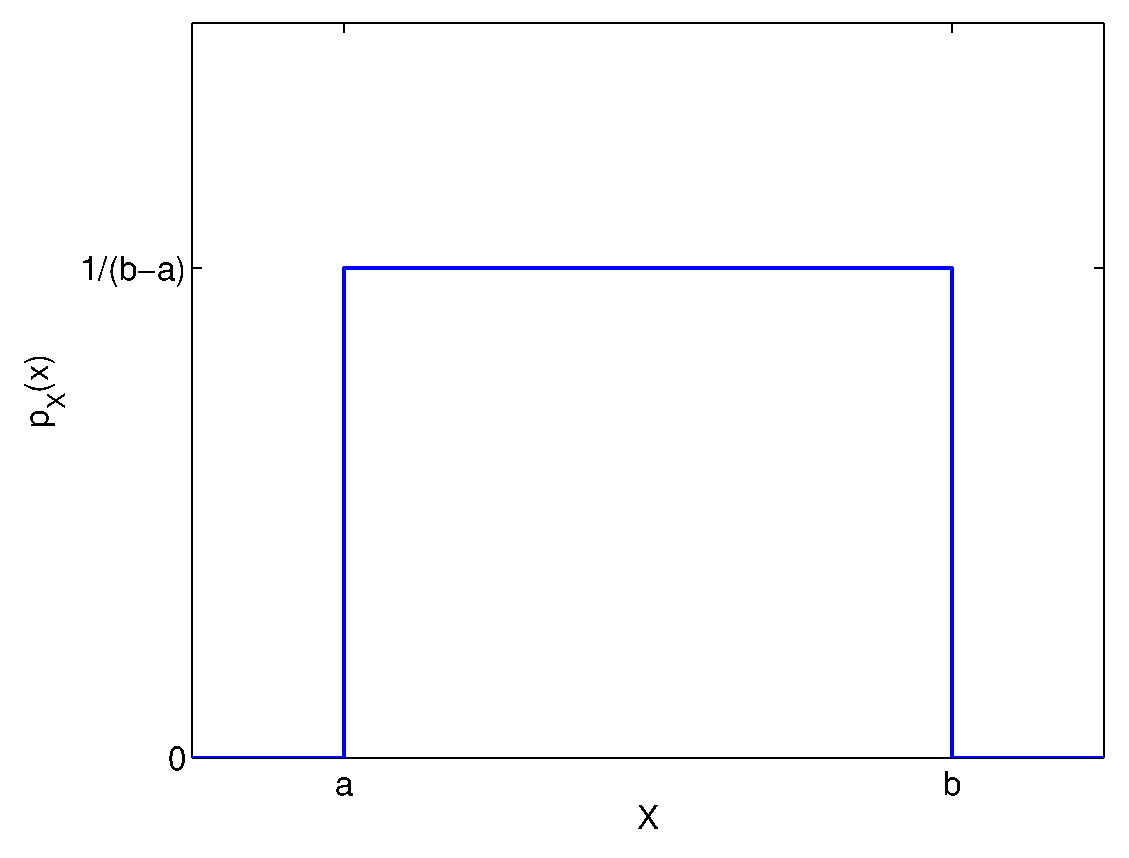
\includegraphics[width=3.5cm]{./Figures/ProbUniforme.eps}
\end{frame}


\begin{frame}\frametitle{Variables aleatorias comunes}
  \begin{itemize}
    \item \alert{Distribución gaussiana}:\hspace{0.2cm}
    \small$p_X(x)=\mathcal{N}_{X}(x;\mu,\sigma)=\frac{1}{\sqrt{2\pi \sigma^2}} e^{-\frac{(x-\mu)^2}{2\sigma^2}}$
    \begin{itemize}
      \footnotesize
      \item \color{blue}$\mu_x=\int_{-\infty}^{\infty}x p_X(x)dx=\mu$\color{black}
      \vspace{0.1cm}
      \item \color{blue}$E(X^2)=\int_{-\infty}^{\infty}x^2 p_X(x)dx=\sigma^2+\mu_x^2$\color{black}
      \vspace{0.1cm}
      \item \color{blue}$\sigma^2_X=E(X^2)-\mu^2_X=\sigma^2$\color{black}
      \vspace{0.1cm}
    \end{itemize}
  \end{itemize}
  \centering
  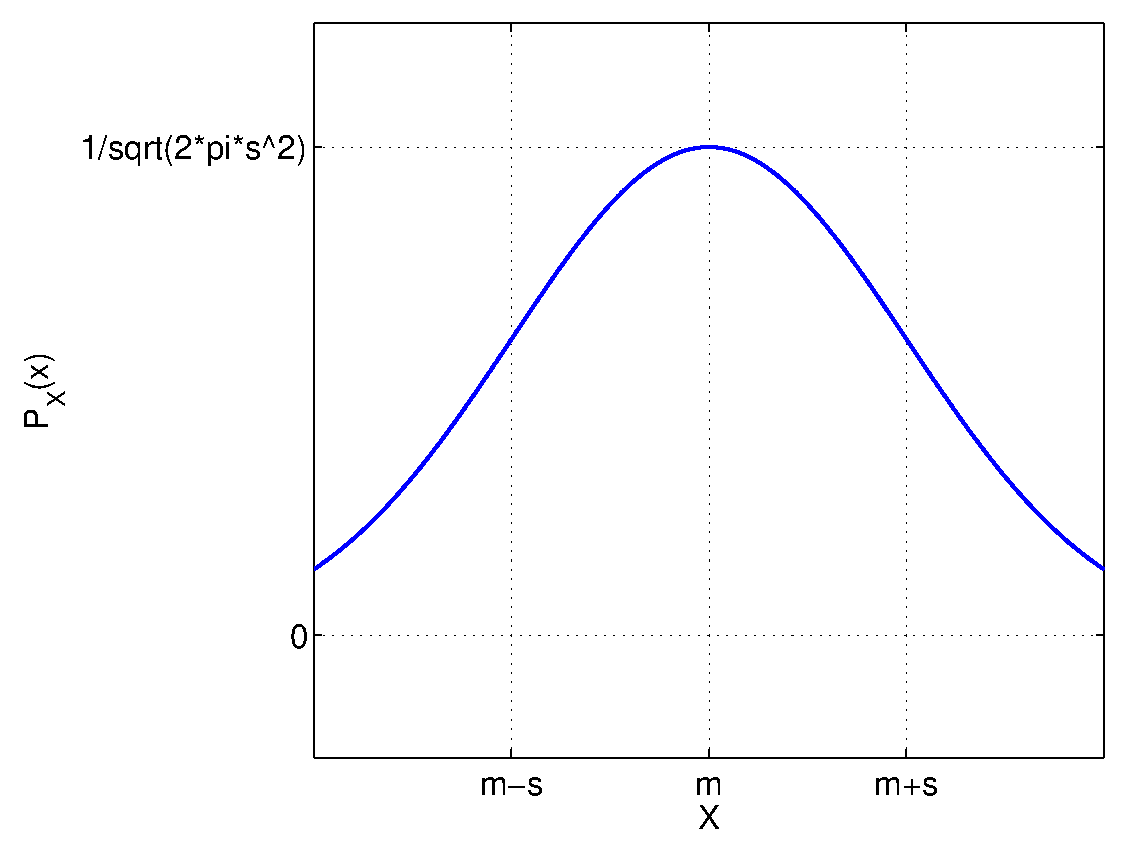
\includegraphics[width=3.5cm]{./Figures/ProbGauss.eps}
\end{frame}
    



\begin{frame}
\frametitle{Muestreo de una variable aleatoria I}

\footnotesize

\begin{itemize}
  \item \alert{Muestreo de una variable aleatoria:}
  \begin{itemize}\scriptsize
    \item Obtener sus valores (muestras) de acuerdo con la densidad de probabilidad.
    \item Matemáticamente representaremos la función como: \color{olivegreen}$x \sim p_X(x)$\color{black}
  \end{itemize}  
  \item \alert{¿Cómo generar las muestras?}
  \begin{itemize}\scriptsize
    \item  Experimentalmente, excitando/observando la respuesta 
    \begin{itemize}\scriptsize
      \item de un proceso aleatorio 
      \item de un proceso determinista con una entrada aleatoria
    \end{itemize}
    \item Utilizando un generador de números pseudo-aleatorios:

    \begin{itemize}\scriptsize
      \item Probabilidad \alert{discreta}: \color{blue}$p_x(x_i)$ con $i\in [1:N]$\color{black}\\\scriptsize
      \color{blue}$\bullet\:\:$\color{black} Equiprobables con Matlab: \color{blue}\texttt{randi($\#_{valores}$,filas,col)}\color{black}\\
      \color{blue}$\bullet\:\:$\color{black} No equiprobables: método de la ruleta
      \item Probabilidad \alert{uniforme}: \color{blue}$\mathcal{U}_{X\in [a,b]}(x)$\color{black}\\\scriptsize
      \color{blue}$\bullet\:\:$\color{black} Matlab: \color{blue}\texttt{a+(b-a)*rand(filas,col)}\color{black}\\
      \color{blue}$\bullet\:\:$\color{black} Secuencias básicas: $x_{i+1}=(a*x_i+c)\mod m$.
      \hspace{3.2cm}\color{gray}{Ejemplo con $a=65539, m=2^{29}$}\color{black}
      \item Probabilidad \alert{gaussiana}: \color{blue}$\mathcal{N}_{X}(x;\mu,\sigma)$\color{black}\\\scriptsize
      \color{blue}$\bullet\:\:$\color{black} Matlab: \color{blue}\texttt{$\mu$+$\sigma$*randn(filas,col)}\color{black}\\
      \color{blue}$\bullet\:\:$\color{black} Transformada de Box-Muller (a partir de la uniforme)
      \item Probabilidades \alert{genéricas}:\\\scriptsize
      \color{blue}$\bullet\:\:$\color{black}Muestreo por rechazo, por importancia\\
      \color{blue}$\bullet\:\:$\color{black} Muestreo de mezclas
    \end{itemize}
    \end{itemize}
  \end{itemize}
\end{frame}

\begin{frame}
\frametitle{Muestreo de una variable aleatoria II}

\footnotesize


\begin{columns}[T]
\begin{column}{7cm}
\begin{itemize}
\item \alert{Método de la ruleta:}
\begin{itemize}
\footnotesize
\item $p(x_i)$
\item Muestreo variable auxiliar:
$y \sim \mathcal{U}_{y\in [0,1]}(y)$
\item $x=\{ j |\sum_{i=1}^{j-1}p(x_i) < y<\sum_{i=1}^j p(x_i)\}$
\end{itemize}
 \end{itemize}
\end{column}
\begin{column}{4cm}
\visible<2->{
\lstinputlisting{./Matlab/Ruleta.m}
}
\end{column}
\end{columns}

\vspace{-0.2cm}

\visible<3->{

\begin{columns}[T]
\begin{column}{7cm}
\begin{itemize}
\item \alert{Transformada de Box-Muller:}
\begin{itemize}
\footnotesize
\item  $\mathcal{N}(x,\mu\!=\!0,\sigma^2\!=\!1)$
\item Muestreo de 2 variables auxiliares:

\hspace{0.3cm}$y_1 \sim \mathcal{U}_{y\in [0,1]}(y)$

\hspace{0.3cm}$y_2 \sim \mathcal{U}_{y\in [0,1]}(y)$
\item Transformación de las muestras:

\hspace{0.3cm}$r=\sqrt{-2\log(y_1)}$

\hspace{0.3cm}$\theta=2\pi y_2$

\hspace{0.3cm}$x_1=r \cos(\theta)$

\hspace{0.3cm}$x_2=r \sin(\theta)$

\scriptsize
Se genera un par, para hacer una guassiana de dos dimensiones o un complejo. Se puede usar solo uno.
\end{itemize}
 \end{itemize}

\end{column}
\begin{column}{4cm}
\visible<4->{
\lstinputlisting{./Matlab/BoxMuller.m}}
\end{column}
\end{columns}

}


 \end{frame}

%%%%%%%%%%%%%%%%%%%%%%%%%%%%%%%%%%%%%%%%%%%%%%%%



\begin{frame}
\frametitle{Muestreo de una variable aleatoria III}

\footnotesize


\begin{columns}[T]
\hspace{-0.5cm}\begin{column}{7cm}
\begin{itemize}
\item \alert{Método de muestreo por rechazo:}
\begin{itemize}
\footnotesize
\item Función de probabilidad genérica $p(x)$
\item Las muestras se obtienen de una $q(x)$ auxiliar que debe cumplir que para algún M que Mq(x)-p(x)>0.  Este hecho fuerza a que tengan el mismo soporte (que $q(x)\ne 0$ sobre los mismos puntos x que $p(x)\ne 0$).
\item Las $x\sim q(x)$ son también muestras de $p(x)$ si se cumple que $yMq(x)<p(x)$ con $y \sim \mathcal{U}_{y\in [0,1]}(y)$
\end{itemize}
 \end{itemize}


 \hspace{2cm}\includegraphics[width=3.5cm]{./Figures/MuestreoRechazo.eps}

\end{column}
\begin{column}{4,5cm}

\visible<2->{

\lstinputlisting{./Matlab/MuestreoRechazo.m}}
\end{column}
\end{columns}

\vspace{-0.2cm}



 \end{frame}


%%%%%%%%%%%%


\begin{frame}
\frametitle{Muestreo de una variable aleatoria IV}

\footnotesize


\begin{columns}[T]
\begin{column}{6.8cm}
\begin{itemize}
\item \alert{Muestreo de una mezcla:}
\begin{itemize}
\footnotesize
\item Función de probabilidad genérica $p(x)=\sum_{i=1}^La_ip_i(x)$, con $\sum_{i=1}^L a_i=1$
\item Para muestrearla, podemos seguir el siguiente proceso:
\begin{itemize}
\item Elegimos la componente de la mezcla (el valor de la i) utilizando la probabilidad discreta $q(i)=a_i$
\item Muestreamos la x de la componente elegida $x \sim p_i(x)$
\end{itemize}
\end{itemize}
 \end{itemize}

\visible<2->{
 \hspace{2cm}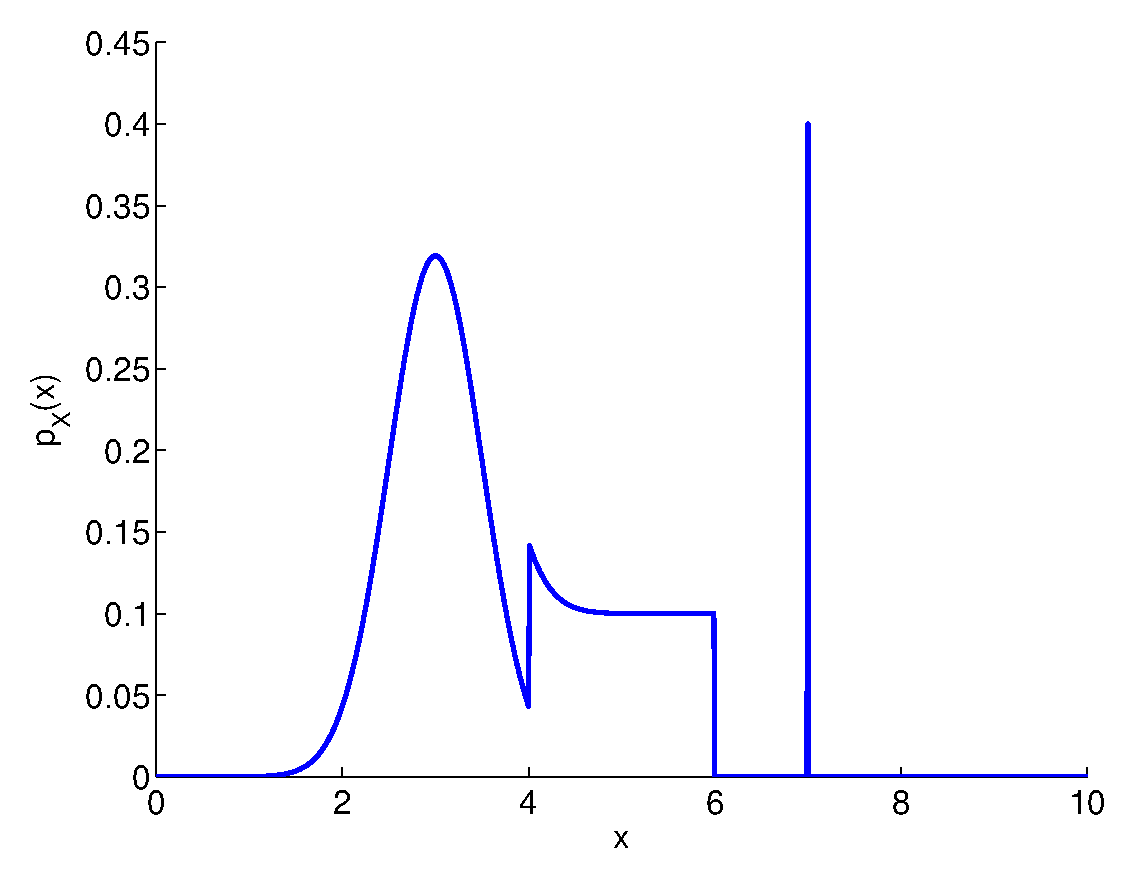
\includegraphics[width=3.5cm]{./Figures/MuestreoMezcla.eps} }

\end{column}
\begin{column}{4.2cm}

\visible<3->{

\lstinputlisting{./Matlab/MuestreoMezcla.m}
}

\visible<2->{
\small
\color{olivegreen}

$p_X(x)=0.4\mathcal{N}(x,3,0.5)+$


\hspace{1.35cm}$0.2\mathcal{U}_{[4,6]}(x)+$

\hspace{1.35cm}$0.4\delta(x-7)$

}
\end{column}
\end{columns}

\vspace{-0.2cm}
 \end{frame}


\begin{frame}
\frametitle{Caracterización de las muestras}

\footnotesize

\vspace{-0.2cm}

\begin{itemize}
\item ¿Que hacer cuando nos proporcionan un conjunto de muestras sin su función de probabilidad?

\visible<2->{

\item El proceso de caracterización de las muestras es conceptualmente análogo al proceso de caracterización de la función de probabilidad. }

\visible<3->{
\item La diferencia reside que en el primer caso no se dispone de una función de probabilidad y en el segundo si.
}

\visible<4->{

\item En el proceso de caracterización de las muestras se puede:
}
\begin{itemize}
\footnotesize

\visible<5->{


\item Intentar estimar la función de probabilidad:
\begin{enumerate}
\item Determinar el tipo de función de probabilidad: histograma de las muestras
\item Determinar los parámetros de la función de probabilidad: a partir de las muestras
\end{enumerate}
}

\visible<6->{

\item Obtener el valor de los estadísticos a partir:
\begin{itemize}
\item De la muestras: Método de Monte-Carlo$^1$
\item De la función de probabilidad que se ha estimado.
}
\end{itemize}
\end{itemize}

\end{itemize}

\vspace{-0.3cm}


\visible<7->{

\rule{11cm}{0.04ex}
\scriptsize

$^1$Los métodos de Monte-Carlo también se utilizan para estimar los estadísticos de funciones de probabilidad conocidas de las que no se pueden calcular las integrales de forma cerrada. El proceso consiste en utilizar los métodos de muestreo para generar muestras de la función de probabilidad y luego el método de Monte-Carlo para estimar el estadístico sobre las muestras generadas.
}
\end{frame}

%%%%%%%%%%%%%%%%%%%%%%%%%%%%%%%%%%%%%%%%%%%%%%

\begin{frame}
\frametitle{Histograma de un conjunto muestral I}

\vspace{-0.3cm}

\footnotesize

\begin{columns}[T]
\hspace{0.2cm}\begin{column}{6cm}
\begin{itemize}
\item El histograma divide el espacio muestral en H segmentos (cubos/bins) continuos de igual tamaño y contabiliza el número de muestras que pertenecen a cada uno de los segmentos.
\end{itemize}
\end{column}
\begin{column}{5cm}
 \hspace{2cm}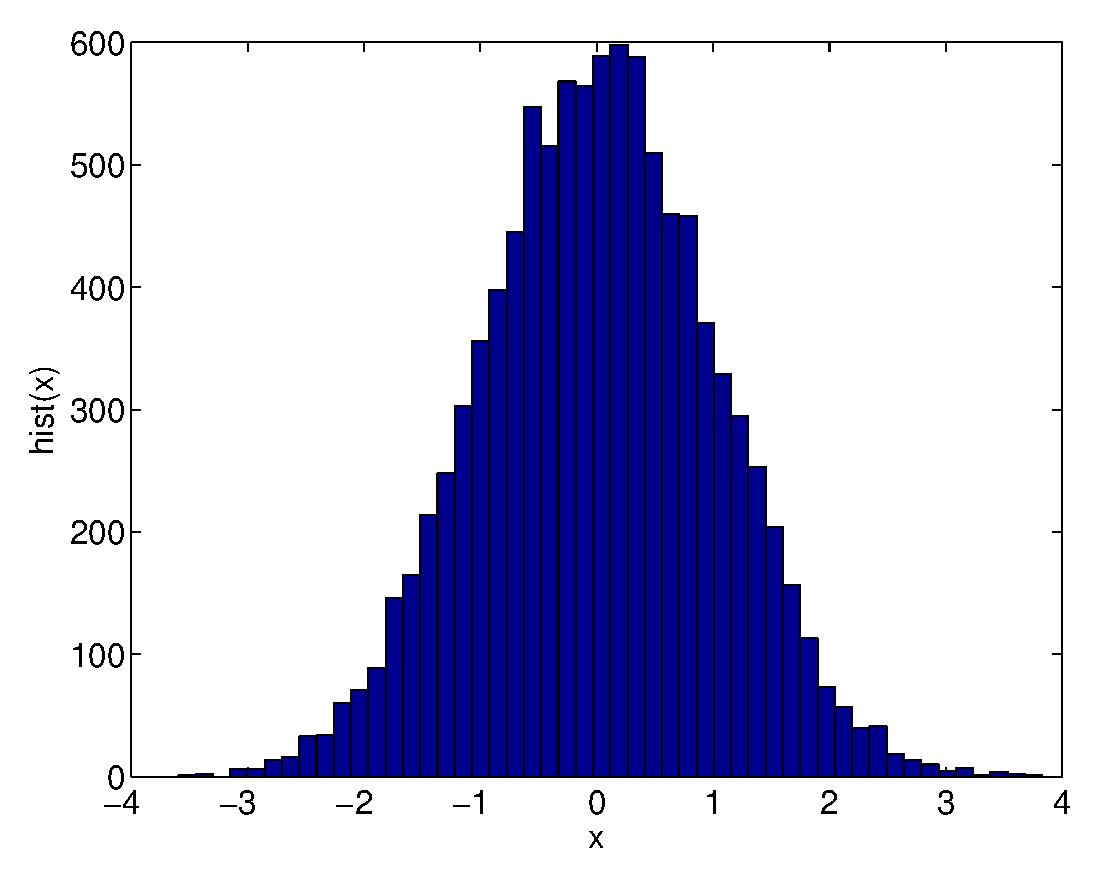
\includegraphics[width=3.1cm]{./Figures/Histograma1.eps}
\end{column}
\end{columns}

\vspace{-0.1cm}

\begin{itemize}

\visible<2->{


\item Podemos utilizarlos para realizar una representación aproximada de la probabilidad de las muestras, siempre y cuando se normalizan las cuentas del histograma de forma que:

\vspace{-0.1cm}

\begin{itemize}
\footnotesize
\item La suma de los valores normalizados del histograma sea 1 para el caso de trabajar con variables aleatorias discretas.
\item El area recogida por el histograma normalizado sea igual a 1 para el caso de trabajar con variables aleatorias continuas.
 \end{itemize}
}
 \vspace{-0.2cm}

\visible<3->{


 \item Una análisis de la forma del histograma (o del histograma normalizado), en la que obviemos los escalones introducidos por la segmentación del espacio muestral, nos puede permitir determinar en algunos casos el tipo de función de probabilidad al que pertenecen las muestras$^1$.

 }
\end{itemize}

\vspace{-0.4cm}


\visible<4->{
\rule{11cm}{0.04ex}
\scriptsize

$^1$En el caso continuo, es conveniente hacer divisiones suficientemente pequeñas para que los escalones no escondan la función de probabilidad real de las muestras.
}
\end{frame}

%%%%%%%%%%%%%%%%%%%%%%%%%%%%%%%%%%%%%%%%


\begin{frame}
\frametitle{Histograma de un conjunto muestral II}
\footnotesize

\begin{columns}[c]
\begin{column}{6.5cm}

\scriptsize

\vspace{-0.2cm}

\color{olivegreen}Ejemplo: Histograma de muestras  $\sim \mathcal{N}_X(x,0,1)$\color{black}

\vspace{-0.2cm}

\lstinputlisting{./Matlab/HistNormal.m}

\end{column}
\begin{column}{4.5cm}
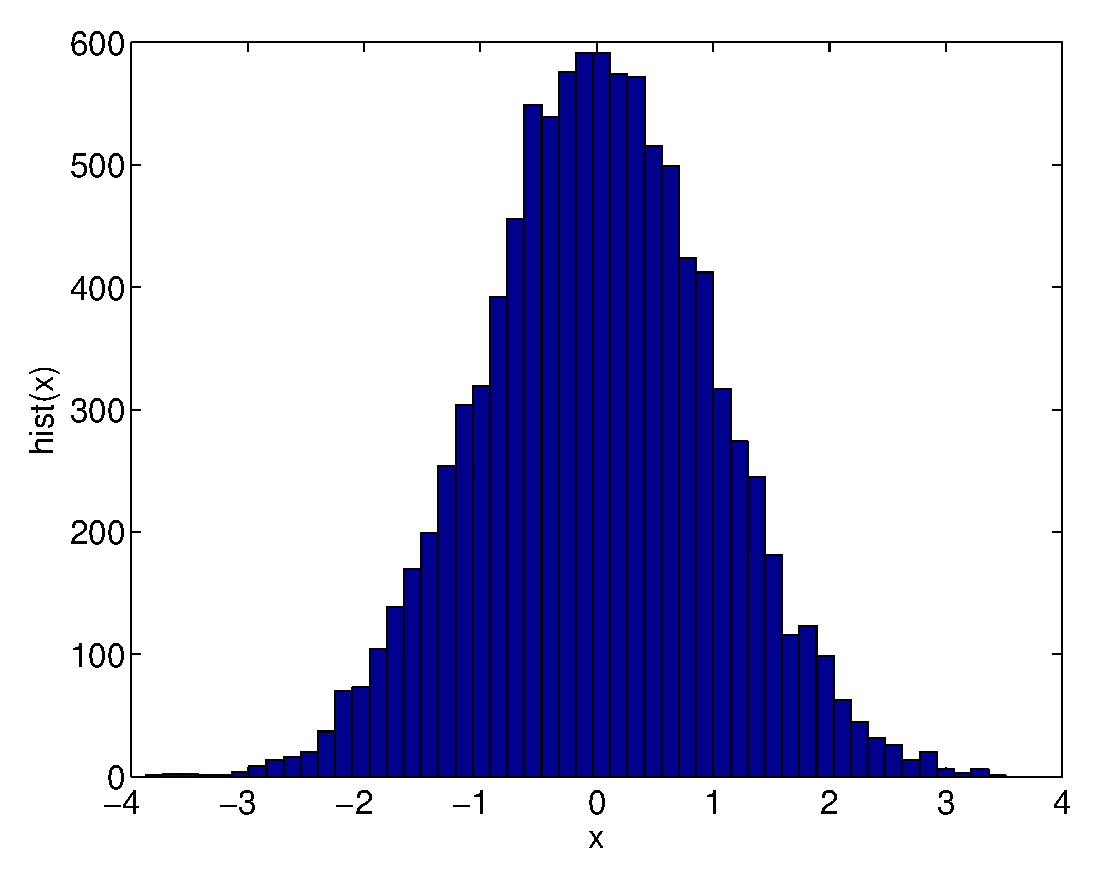
\includegraphics[width=3cm]{./Figures/HistNormal1.eps}

\visible<2->{
\vspace{-1.6cm}
\hspace{1cm}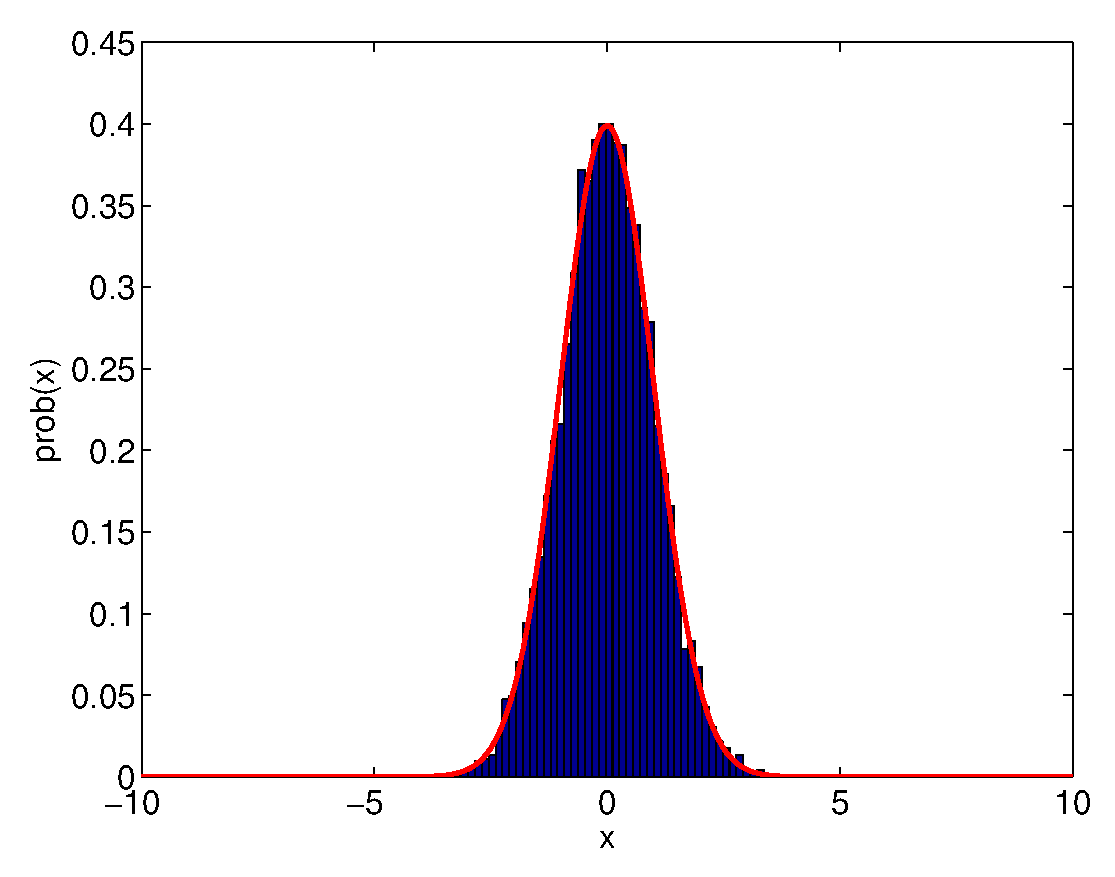
\includegraphics[width=3.5cm]{./Figures/HistNormal2.eps}
}

\end{column}
\end{columns}

% \vspace{0.3cm}

\begin{columns}[c]
\begin{column}{6cm}

\scriptsize
\centering

\visible<3->{

\color{olivegreen}Histograma del ejemplo del rechazo\color{black}

\vspace{0.2cm}

\only<3|handout:0>{\includegraphics[width=4cm]{./Figures/MuestreoRechazo.eps}}\only<4->{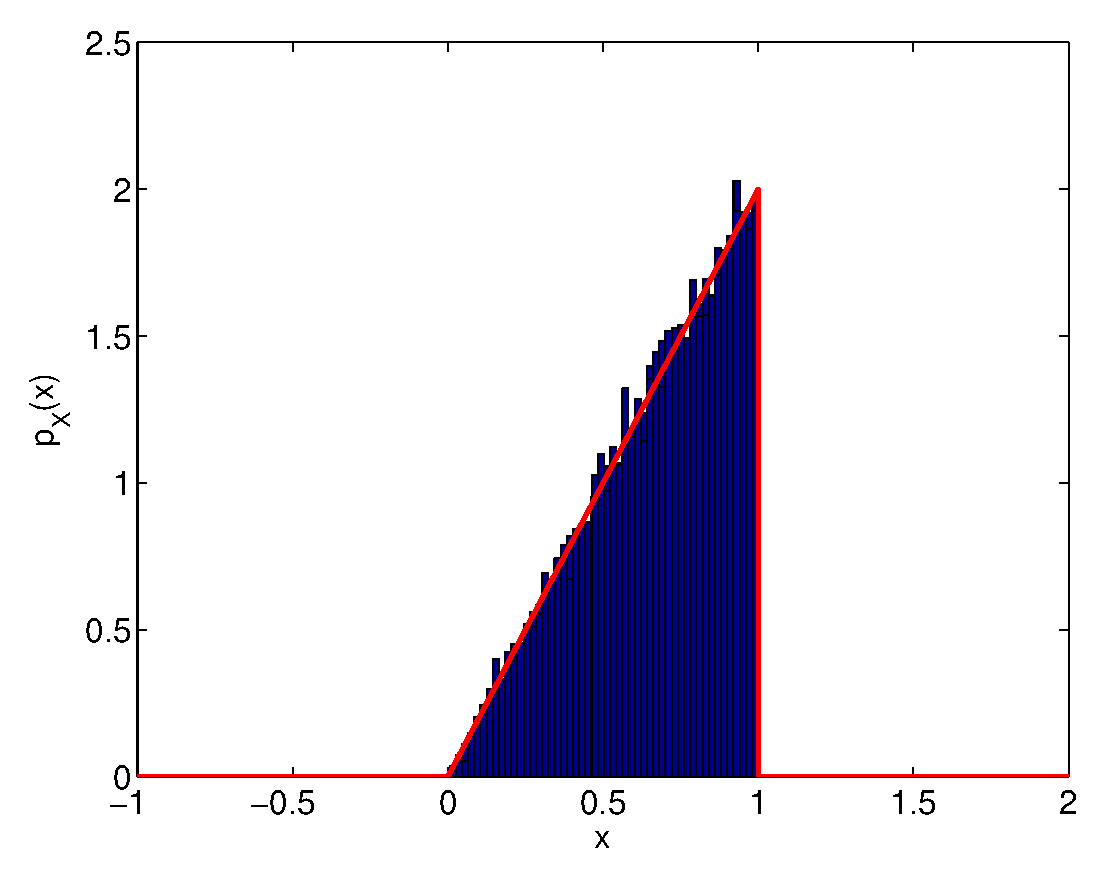
\includegraphics[width=4cm]{./Figures/HistRechazo.eps}}
}



\end{column}
\begin{column}{6cm}
\scriptsize
\centering

\visible<5->{

\color{olivegreen}Histograma del ejemplo de la mezcla\color{black}

\vspace{0.2cm}
\only<5|handout:0>{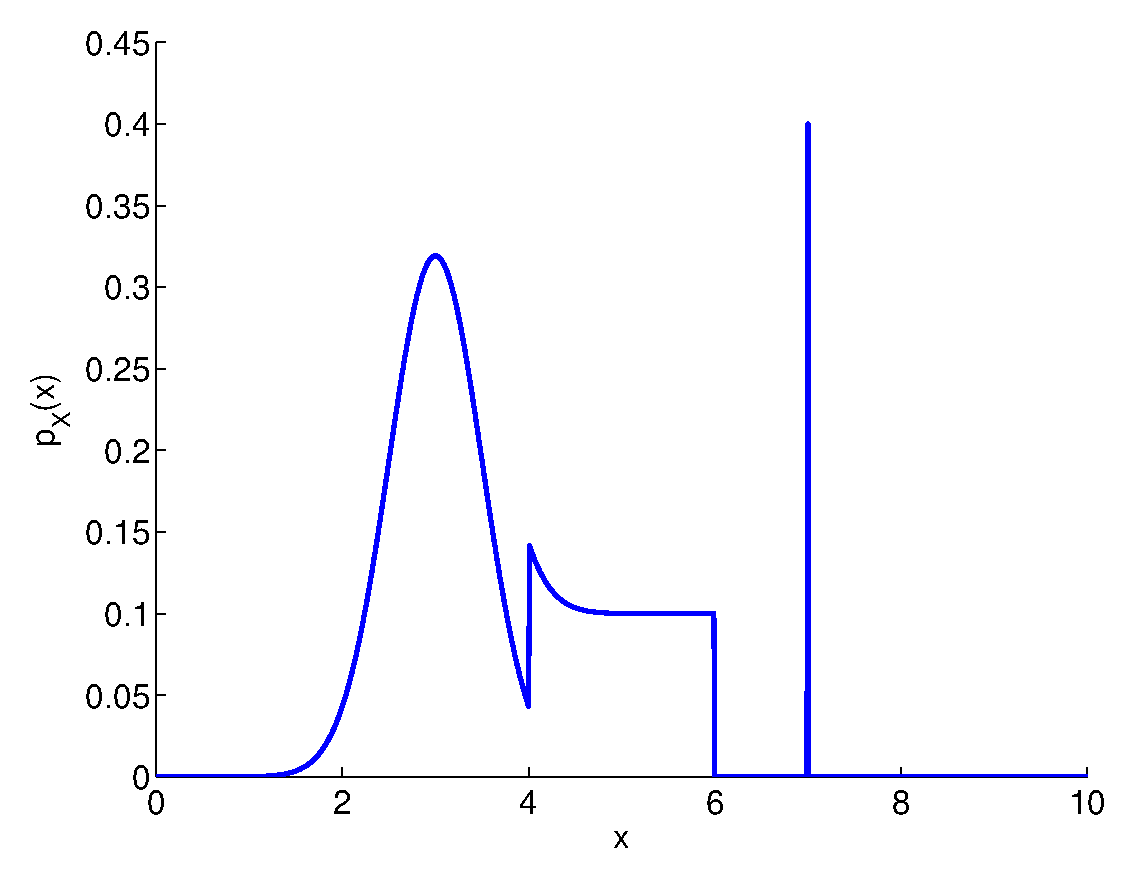
\includegraphics[width=4cm]{./Figures/MuestreoMezcla.eps}}\only<6->{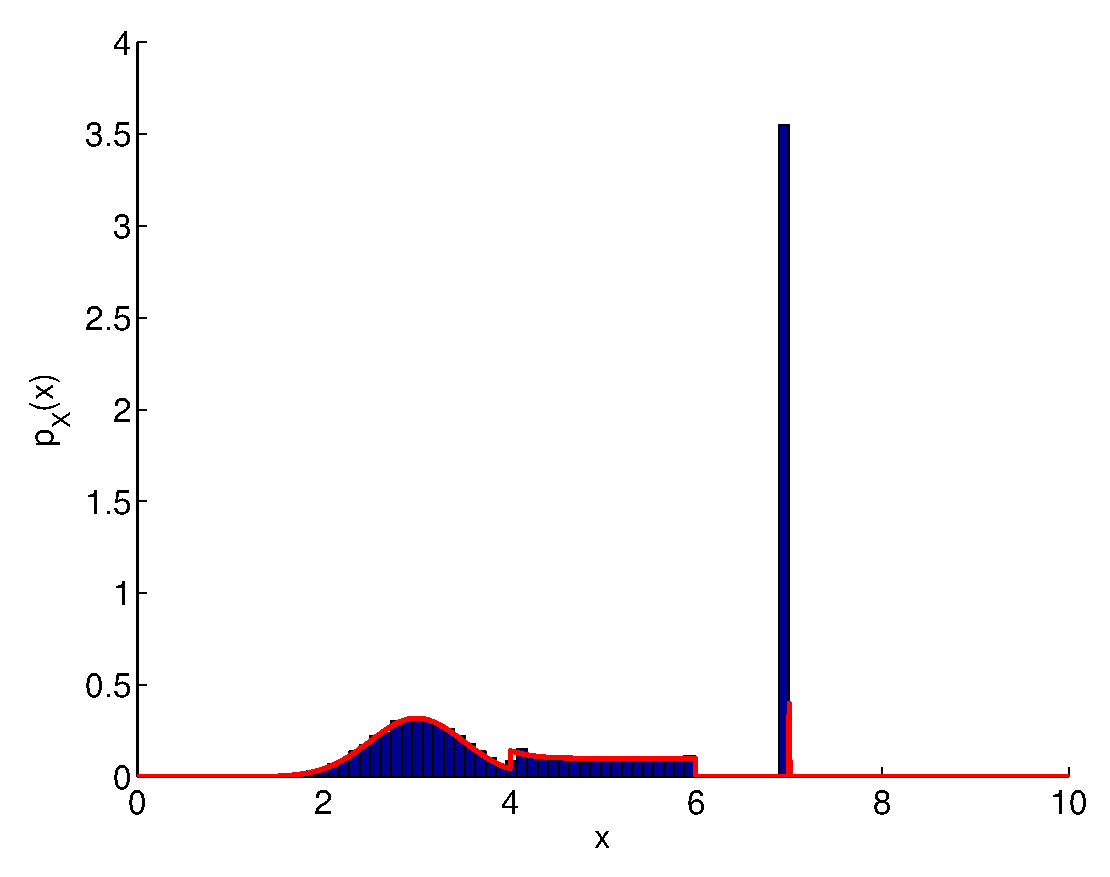
\includegraphics[width=4cm]{./Figures/HistMezcla.eps}}
}

\end{column}
\end{columns}

\end{frame}

%%%%%%%%%%%

\begin{frame}
\frametitle{Métodos de Monte-Carlo}
\footnotesize

\begin{itemize}
\item ¿Como podemos estimar el valor de los estadísticos a partir de las muestras directamente?

\visible<2->{

\item Podemos aproximar  la probabilidad que representan las $N$ muestras por: $p_X(x)=\frac{1}{N}\sum_{n=1}^{N} \delta(x-x_i)$.}

\visible<3->{

\item A partir de esa fórmula, podemos obtener los estadísticos directamente:}
\begin{itemize}
\footnotesize
\visible<3->{

\item  $E(g(X))\!=\!\!\int_{-\infty}^\infty g(x)p_X(x)dx\!=\!\!\int_{-\infty}^\infty g(x) \frac{1}{N}\!\!\sum_{n=1}^{N} \delta(x-x_i) dx\!=$}


\visible<4->{

\vspace{0.1cm}


\hspace{1.15cm}$=\!\frac{1}{N}\sum_{n=1}^{N} \!g(x_i)$

\vspace{0.1cm}


\item Valor medio: $\mu_X=E(X)=\!\frac{1}{N}\sum_{n=1}^{N} \! x_i$

\vspace{0.1cm}


\item Valor cuadrático medio: $E(X^2)=\!\frac{1}{N}\sum_{n=1}^{N} \! x_i^2$

\vspace{0.1cm}


\item Varianza: $\sigma_X^2=E((X-\mu_X)^2)=\!\frac{1}{N}\sum_{n=1}^{N} \! (x_i-\mu_x)^2$
}
\end{itemize}

\visible<5->{

\item Los estadísticos básicos se pueden calcular directamente con Matlab:

\begin{itemize}
\footnotesize
\item Valor medio: \color{blue}\texttt{mu=mean(samples)}\color{black}
\item Varianza$^1$: \color{blue}\texttt{sigma2=var(samples,1)}\color{black}
\item Desviación estandard$^1$ ($\sigma_X$): \color{blue}\texttt{sigma=std(samples,1)}\color{black}
\end{itemize}
}

\end{itemize}

\vspace{-0.2cm}

\visible<5->{


\rule{11cm}{0.04ex}
\scriptsize
$^1$El segundo parámetro tiene que tomar el valor de 1 para que se calcule la varianza dividiendo los resultados entre N.
}

\end{frame}

 %%%%%%%%%%%%%%Empieza la presentacion%%%%%%%%%%%%%%%%%%%%%%%%%%%%%%%%%%%%


%%%%%%%%%%%%%%%%%%%%%%%%%%%%%%%%%%%%
%%%%%%%%%%%%%%%%%%%%%%%%%%%%%%%%%%%%

\subsection{Múltiples variables aleatorias}



\begin{frame}
\frametitle{Definición de múltiples variables aleatorias I}

\vspace{-0.2cm}

\footnotesize

\begin{itemize}
\item Las propiedades de un conjunto $\{X_1,X_2,\dots,X_M\}$ de variables aleatorias se definen a través de la función probabilidad$^1$ conjunta $p_{\{X_1,X_2\dots,X_M\}}(x_1,x_2,\dots,x_M)$.

\vspace{0.1cm}

\item Las probabilidad conjunta se refiere al hecho de la probabilidad de la variable $X_1$ se encuentre en el estado $x_1$ y la variable $X_2$ se encuentre en el estado $x_2$ ... y la variable $X_M$ se encuentre en el estado $x_M$.

\visible<2->{

\item Operaciones básicas de probabilidades:

}
\begin{itemize}
\footnotesize

\visible<2->{

\item Regla de la cadena (existen $M!$ factorizaciones posibles): 


\hspace{0.2cm}{\scriptsize$p_{\{X_1,\dots,X_M\}}(x_1,\dots,x_M)=p_{X_1}(x_1|x_2,\dots,x_M)p_{X_2}(x_2|x_3,\dots,x_M)\cdots p_{X_M}(x_M)$}
}
\vspace{0.1cm}

\visible<3->{

\item Independencia condicional de $X_a$ de $X_b$ dados los valores de $\{x_1,\dots,x_L\}$:

\hspace{0.2cm}$p(x_a|x_1,\dots,x_L,x_b)=p(x_a|x_1,\dots,x_L)$
}

\visible<4->{

\item Independencia condicional de un conjunto de variables$^2$:

\vspace{0.1cm}

\hspace{0.2cm}$p_{\{X_1,\dots,X_M\}}(x_1,\dots,x_M)=\prod_{i=1}^M p_{X_i}(x_i)$

}

\end{itemize}


\end{itemize}

\vspace{-0.3cm}

\rule{11cm}{0.04ex}
\scriptsize
$^1$Aunque la definición de las variables aleatorias puede realizarse, al igual que en el caso de continuos, a través de diferentes funciones de probabilidad, vamos a utilizar la definición de probabilidad de masa y densidad de probabilidad.

\visible<4->{


\vspace{0.1cm}

$^2$La expresión se obtiene a partir de la regla de la cadena y aplicando el hecho de que son probabilisticamente independientes todas de todas. 
}

\end{frame}

%%%%%%%%%%%%%%%%%

\begin{frame}
\frametitle{Definición de múltiples variables aleatorias II}

\footnotesize


\begin{itemize}
\item Operaciones básicas de probabilidades conjuntas:
\begin{itemize}
\footnotesize

\visible<2->{


\item Marginalización (probabilidad de un subconjunto):

\begin{itemize}

\item Variables discretas: $p_{X_1}(x_1)=\sum_{x_2\in X_2} p_{\{X_1,X_2\}}(x_1,x_2)$
\item Variables continuas: $p_{X_1}(x_1)=\int_{-\infty}^{\infty} p_{\{X_1,X_2\}}(x_1,x_2)dx_2$

\end{itemize}
}

\visible<3->{

\item Teorema Bayes$^1$: $p_{X_1}(x_1|x_2)=\frac{p_{X_2}(x_2|x_1)p_{X_1}(x_1)}{p_{X_2}(x_2)}$
}

\end{itemize}


\end{itemize}

\visible<4->{


\color{olivegreen}{Ejemplo continuo}: Representar la distribución conjunta de las variables $\{X_1,X_2\}$ a partir de 
$p_{X_1}(x_1)=\mathcal{U}_{[2,4]}(x_1)$ y la $p_{X_2}(x_2|x_1)=\mathcal{N}(x_2;x_1,1)$
}

\color{gray}

\vspace{-0.3cm}

\begin{columns}[c]
\begin{column}{5.5cm}

\visible<5->{


\scriptsize

$p_{X_1}(x_1)=\left \{\begin{array}{ll}\frac{1}{4-2}&\:\: 2\le x_1\le 4\\0 &\:\:c.c. \end{array} \right .$

\vspace{0.1cm}

$p_{X_2}(x_2|x_1)=\frac{1}{\sqrt{2\pi}}e^{-\frac{(x_2-x_1)^2}{2}}$


\vspace{0.2cm}

$p_{\{X_1,X_2\}}(x_1,x_2)=p(x_2|x_1)p(x_1)=$

\hspace{0.4cm}$=\left \{\begin{array}{ll}\frac{1}{2\sqrt{2\pi}}e^{-\frac{(x_2-x_1)^2}{2}}&\:\: 2\le x_1\le 4\\0 &\:\:c.c. \end{array} \right .$
}
\end{column}
\hspace{-1.5cm}\begin{column}{6.3cm}


\visible<6->{

\lstinputlisting{./Matlab/ProbConjunta.m}}

\visible<7->{


\vspace{-1.0cm}
\hspace{3.3cm}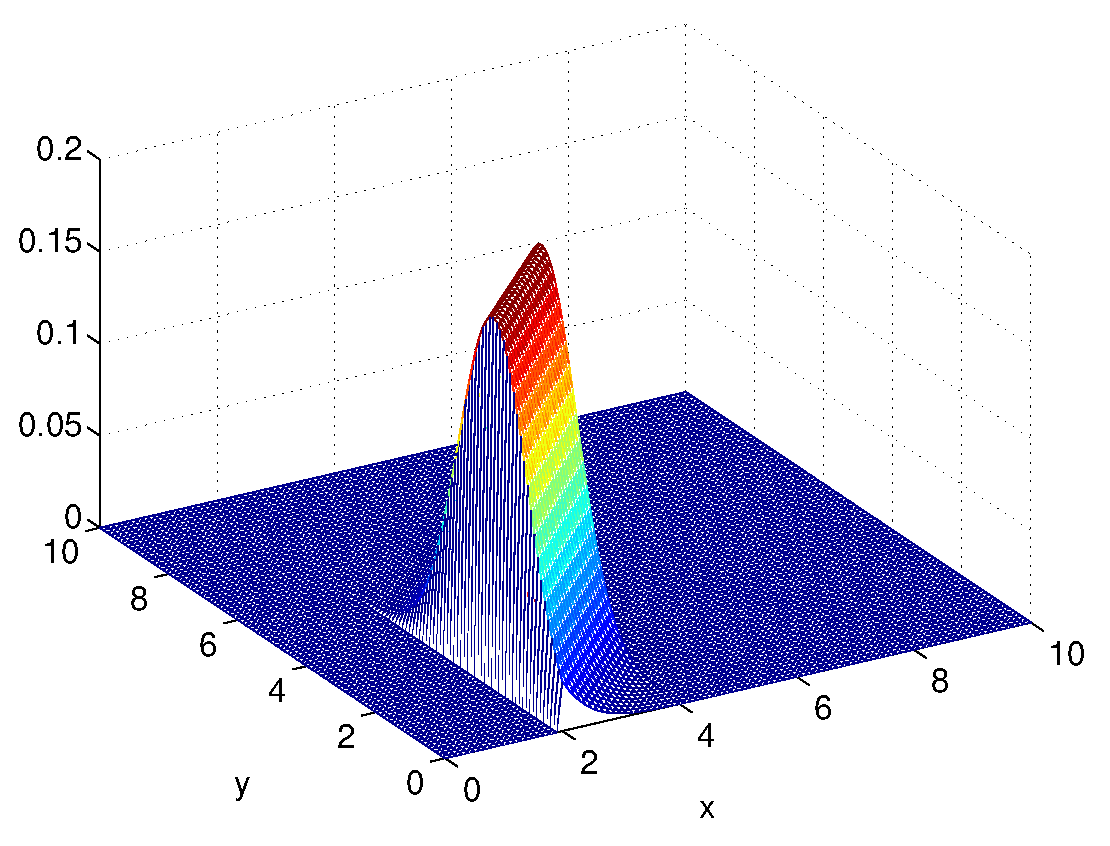
\includegraphics[width=3cm]{./Figures/ProbConjunta.eps} 

}



\end{column}
\end{columns}

\vspace{0.0cm}



\color{black}
\visible<3->{


\rule{11cm}{0.04ex}
\scriptsize
$^1$Se puede derivar a partir de la regla de la cadena para un conjunto de dos variables: $p(x_1,x_2)=p(x_1|x_2)p(x_2)=p(x_2|x_1)p(x_1)$
}

\end{frame}


%%%%%%%%%%%%%%%%%%%%%%%%%%%%%%%%%


\begin{frame}
\frametitle{Estadísticos de conjuntos de variables aleatorias}



\footnotesize

\begin{itemize}

\item Suponemos un conjunto de variables aleatorias $\mathcal{X}=\{X_1,X_2,\dots,X_M\}$ y su función de probabilidad conjunta $p_{\{X_1,X_2\dots,X_M\}}(x_1,x_2,\dots,x_M)$.

\item Los estadísticos que se suelen utilizar son:

\begin{itemize}
\footnotesize

\visible<2->{


\item Los estadísticos de cada variable aleatoria por separado: son los mismos que los de una variable aleatoria (sobre la función de probabilidad marginal asociada a cada variable):

\begin{itemize}
\scriptsize
\item  $p_{X_i}(x_i)\!\!=\!\!\int\!\! \int\!\! \int_{-\infty}^{\infty} p_{\{X_1,X_2\dots,X_M\}}\!(x_1,x_2,\dots,x_M)dx_1\cdots dx_{i-1}dx_{i+1}dx_M$

\vspace{0.1cm}

\item Media: $\mu_{X_i}=E(X_i)=\int_{-\infty}^{\infty}x_i p_{X_i}(x_i)dx_i$

\vspace{0.1cm}

\item Valor cuadrático medio: $E(X_i^2)=\int_{-\infty}^{\infty}x_i^2 p_{X_i}(x_i)dx_i$


\vspace{0.1cm}

\item Varianza: $\sigma_{x_i}^2\!=\!E((X_i\!-\!\mu_{x_i})^2)\!=\!\!\int_{-\infty}^{\infty}\!(x_i\!-\!\mu_{x_i})^2 p_{X_i}(x_i)dx_i\!=\!E(X_i^2)\!-\!\mu_{X_i}^2$

 
\end{itemize}
}

\visible<3->{


\item Aparecen estadísticos de parejas de variables aleatorias (sobre la función de probabilidad marginal de cada par de variables):

\begin{itemize}
\scriptsize
\item  $p_{X_iX_j}(x_i,x_j)\!\!= \int_{-\infty}^{\infty} p_{\mathcal{X}} (x_1,x_2,\dots,x_M)dx_{1:i-1} dx_{i+1:j-1}dx_{j+1:M}$

\vspace{0.1cm}

\item Correlación cruzada: $\phi_{X_iX_j}\!=\!E(X_iX_j)\!=\! \int_{-\infty}^{\infty}\!\! x_i x_j p_{X_iX_j}(x_i,x_j)dx_i dx_j$

\vspace{0.1cm}

\item Covarianza: $\psi_{X_iX_j}=E((X_i-\mu_{X_i})(X_j-\mu_{X_j}))=$

\hspace{0.5cm}$=\int_{-\infty}^{\infty} (x_i-\mu_{x_i}) (x_j-\mu_{x_j}) p_{X_i,X_j}(x_i,x_j)dx_i dx_j=\phi_{X_iXj}-\mu_{X_i}\mu_{X_j}$

\item Coeficiente de correlación: $\rho_{X_iX_j}=\frac{\psi_{X_iX_j}}{\sigma_{X_i}\sigma_{X_j}}$


\end{itemize}
}
 
\end{itemize}
\end{itemize}

\end{frame}
%%%%%%%%%%%%%%%%%%%%%%%%%%%%%%%%%

\begin{frame}
\frametitle{Propiedades de pares de variables aleatorias}

\footnotesize
\begin{itemize}



\item Independencia probabilística:
	$p(x_i,x_j)=p(x_i|x_j)p(x_j)=p(x_i)p(x_j)$

\visible<2->{

\item Independencia lineal o falta de correlación cruzada:  $E(X_i X_j)=\mu_{X_i}\mu_{X_j}$
}

\begin{itemize}
\footnotesize

\visible<3->{


\item Independencia probabilística $\rightarrow$ independencia lineal

\vspace{0.1cm}

$E(X_i X_j)\!=\!\! \int_{-\infty}^{\infty}\!\! x_i x_j p_{X_iX_j}(x_i,x_j)dx_i dx_j\!=\!\!\! \int_{-\infty}^{\infty}\!\! x_i x_j p_{X_i}(x_i)p_{X_j}(x_j)dx_i dx_j\!=\!\mu_{X_i}\mu_{X_j}$
}


\vspace{-0.25cm}

\visible<4->{

\item No hay independencia lineal (o las variables están correlacionadas) $\rightarrow$ hay dependencia probabilística
}

\vspace{0.1cm}


\visible<5->{

\item Por lo tanto, la correlación cruzada de las señales ($E(X_i X_j)\neq \mu_{X_i}\mu_{X_j}$) sirve para determinar la existencia de la dependencia probabilística.
}

\end{itemize}




\visible<6->{
\item Independencia probabilística $\rightarrow$ $\psi_{X_iX_j}=0$ (covarianza nula)
 
 
 }
 
  
 \vspace{-0.1cm}
 
 \begin{itemize}
\visible<6->{
\item $\psi_{X_iX_j}=E(X_i,X_j)-\mu_{X_i}\mu_{X_j}=\mu_{X_i}\mu_{X_j}-\mu_{X_i}\mu_{X_j}$
 }
 
 \vspace{0.1cm}
 
 \visible<7->{
\item  $\psi_{X_iX_j}\ne0$ $\rightarrow$ Hay dependencia probabilística.
}

\end{itemize}

 \visible<8->{

\item Coeficiente de correlación:

\begin{itemize}

\footnotesize
\item Independencia probabilística $\rightarrow$ $\rho_{X_iX_j}=0$ (la covarianza es nula)
\item Dependencia lineal $\rightarrow$ $\rho_{X_iX_j}=\pm 1$
\end{itemize}
}
\end{itemize}

\end{frame}

%%%%%%%%%%%%%%%%%%%%%%%%%%%%%%%%%

\begin{frame}
\frametitle{Variables aleatorias comunes}

\vspace{-0.3cm}

\begin{columns}[T]
\begin{column}{8cm}

\begin{itemize}
\footnotesize
\item Conjunto de variables con una distribución uniforme: $p(x_1,\cdots,x_M)=\prod_{i=1:M} \mathcal{U}_{[a_i,b_i]}(x_i)$
\begin{itemize}
\footnotesize
\item Probabilísticamente independientes.

\item Mismas características individuales.

\item Características de los pares de variables (independencia condicional):

\begin{itemize}

\vspace{-0.1cm}


\item Correlación cruzada: 

\vspace{0.1cm}

$\phi_{X_iX_j}=\mu_{X_i}\mu_{X_j}=\frac{b_i+a_i}{2}\frac{b_j+a_j}{2}$

\vspace{0.1cm}


\item Covarianza: $\psi_{X_iX_j}=0$





\end{itemize}

\end{itemize}
 
\end{itemize}

\end{column}
\begin{column}{3.5cm}

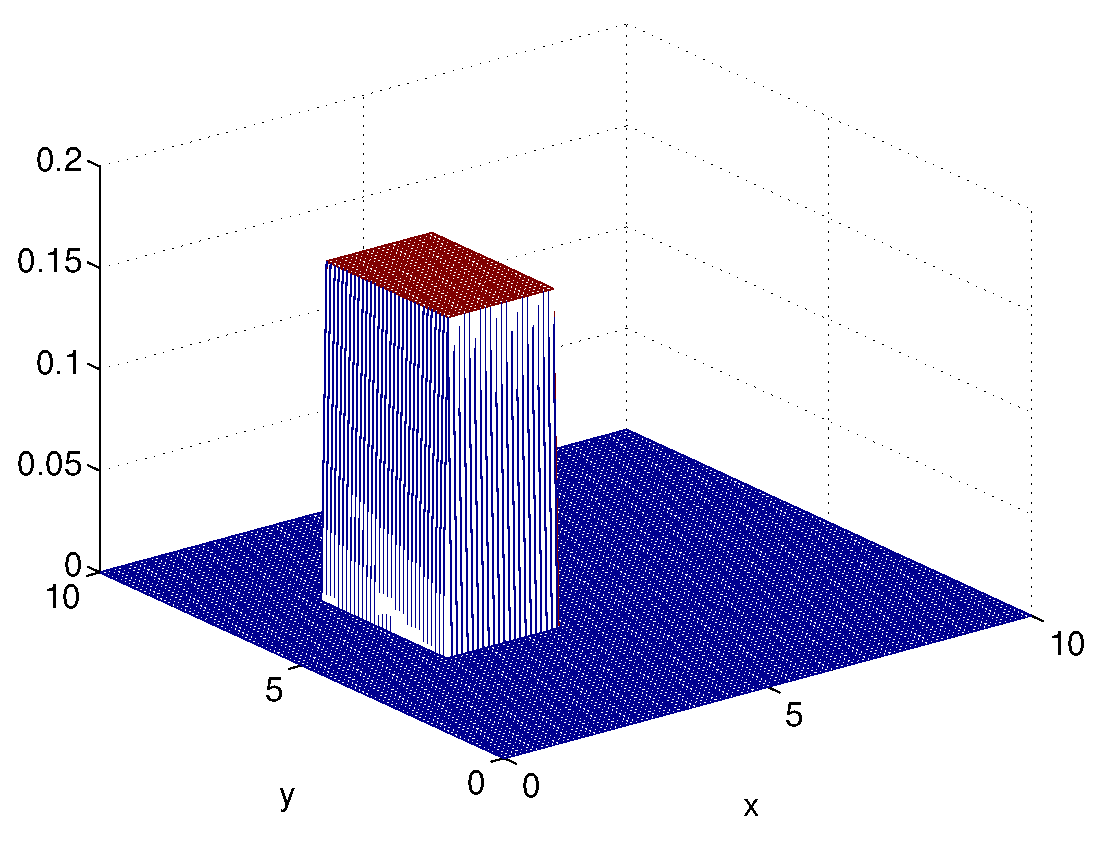
\includegraphics[width=3.5cm]{./Figures/ProbConjuntaUniforme.eps} 

\end{column}
\end{columns}

\visible<2->{

\vspace{-1.1cm}

\begin{columns}[c]
\begin{column}{8cm}

\vspace{0.6cm}

\begin{itemize}
\footnotesize
\item Conjunto de variables ($\bm{x}=[x_1,x_2,\dots,x_M]$) con una distribución gaussiana: $p(x_1,\cdots,x_M)=\frac{1}{\sqrt{(2\pi)^M |\bm{\Sigma}|}}e^{-\frac{1}{2}(\bm{x}-\bm{\mu})\bm{\Sigma}^{-1}(\bm{x}-\bm{\mu})^T}$


\begin{itemize}
\footnotesize

\vspace{-0.1cm}

\item $\bm{\mu}=[\mu_{X_1},\mu_{X_2},\cdots,\mu_{X_M}]$

\vspace{0.2cm}


\item $\bm{\Sigma}=\left[\begin{array}{llll}\sigma^2_{X_1}&\psi_{X_1X_2}&\dots&\psi_{X_1X_M}\\\psi_{X_1X_2}&\sigma^2_{X_2}&\dots&\psi_{X_2X_M}\\ \vdots & \vdots &\ddots & \vdots \\\psi_{X_1X_M}&\psi_{X_2X_M}&\dots&\sigma^2_{X_M}  \end{array}  \right ]$


\end{itemize}
 
\end{itemize}

\end{column}
\begin{column}{3.5cm}



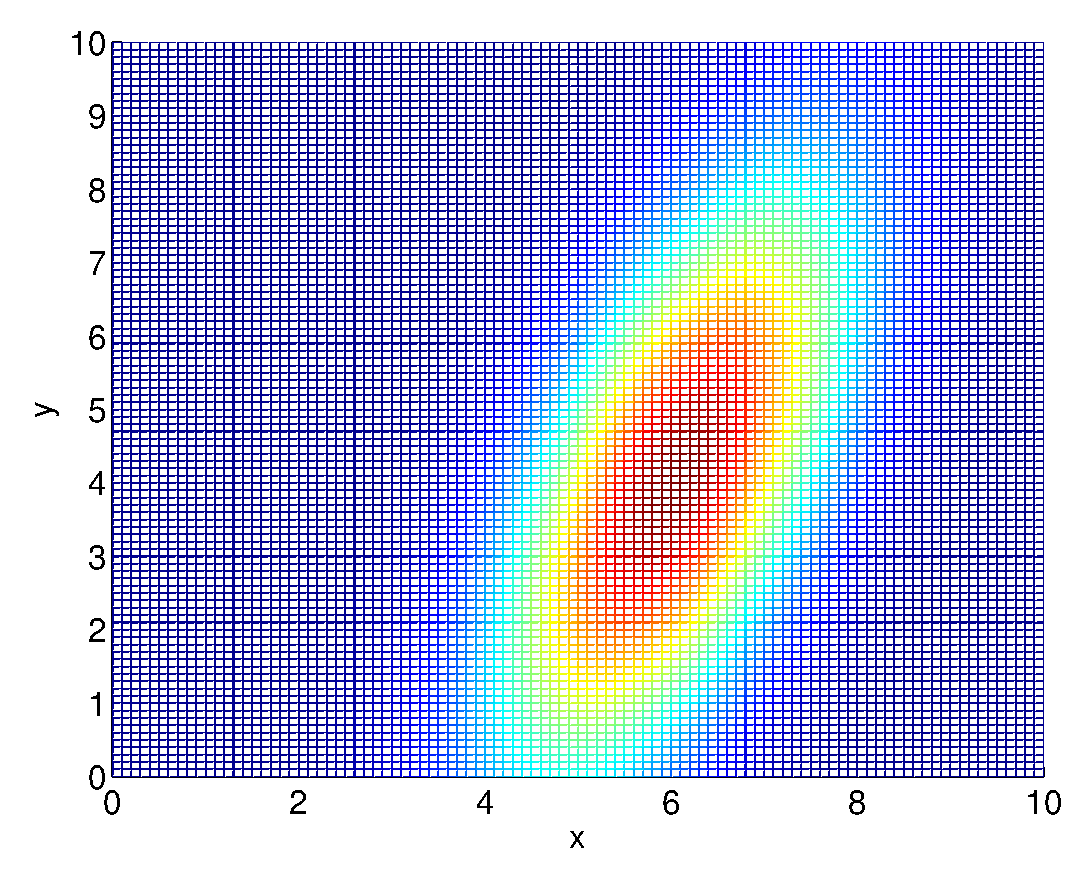
\includegraphics[width=3.1cm]{./Figures/ProbConjuntaGaussiana.eps}

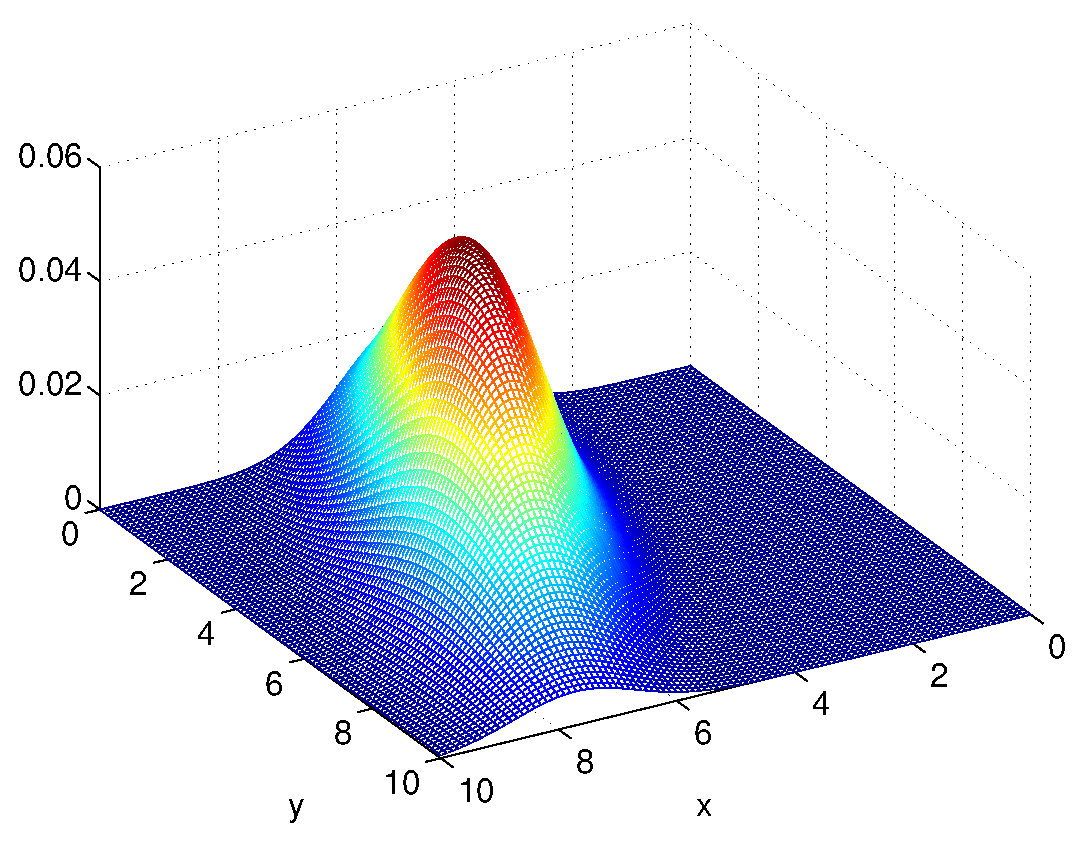
\includegraphics[width=3.5cm]{./Figures/ProbConjuntaGaussiana2.eps} 

\end{column}
\end{columns}
}

\end{frame} 

%%%%%%%%%%%%%%%%%%%%%%%%%%%%%%%%%

\begin{frame}
\frametitle{Variables aleatorias gaussianas}

\vspace{-0.2cm}

\footnotesize

\begin{itemize}
\item La matriz de covarianza $\bm{\Sigma}$ representa un elipsoide M-dimensional, reorientado según los valores de la covarianza que existe entre los diferentes pares de variables.

\item $\bm{\Sigma}$ se puede construir usando la expresión $\bm{\Sigma}=\bm{RDR}'$, donde $\bm{R}$ es una matriz de rotación, y $\bm D$ es una matriz diagonal en la que en cada componente se coloca la varianza asociada a la dirección marcada con la matriz de rotación.

\item Si tenemos la matriz $\bm \Sigma$ podemos calcular la descomposición con la orden de Matlab $\texttt{svd: [R,D]=svd(Sigma)}$.

\end{itemize}

\vspace{-0.5cm}

\begin{columns}[c]
\begin{column}{6cm}

\lstinputlisting{./Matlab/ProbRotacion.m}
\end{column}
\begin{column}{4cm}
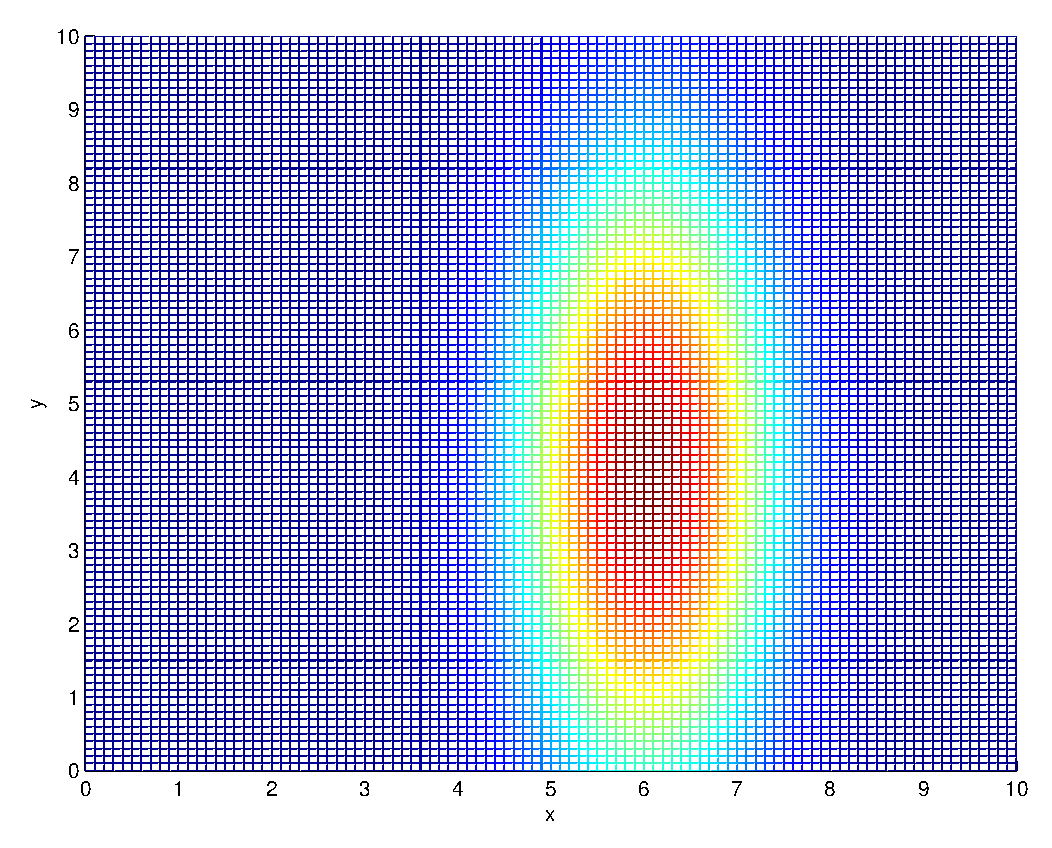
\includegraphics[width=2.8cm]{./Figures/ProbConjuntaGaussiana0.eps} 

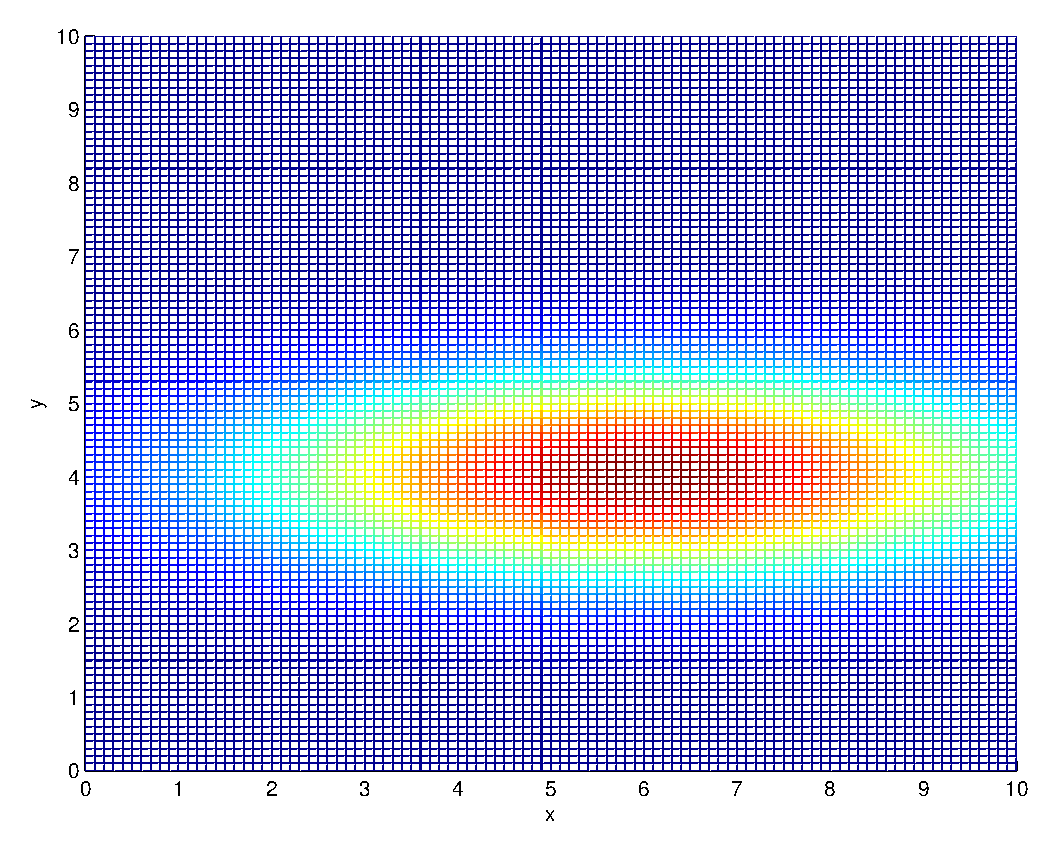
\includegraphics[width=2.8cm]{./Figures/ProbConjuntaGaussiana90.eps} 


\end{column}
\end{columns}

\end{frame}

%%%%%%%%%%%%%%%%%%%%%%%%%%%%%%%%%%%%%%%%%%

\begin{frame}
\frametitle{Muestreo de conjuntos variables aleatorias}

\footnotesize
\begin{itemize}
\item Si tenemos un conjunto de $M$ variables distribuidas uniformemente, podemos aprovechar el hecho de que son independientes condicionalmente las unas de las otras y muestrear cada una de ellas de su distribución uniforme. Una muestra será formada por los conjuntos de $M$ valores muestreados de cada distribución.
\item Si tenemos un conjunto de $M$ variables que tienen una distribución gaussiana conjunta, podemos muestrearlas  a partir de la función randn, teniendo en cuenta el valor medio $\bm{\mu}$ de cada variable y la matriz de covarianza $\bm{\Sigma}=\bm{RDR}'$

\vspace{-0.4cm}

\lstinputlisting{./Matlab/GaussianaN.m}

\item  En el caso de una distribución genérica, se utilizan métodos de simulación de Monte-Carlo. Por ejemplo, se puede hacer un muetreo ordenado, siguiendo una factorización de la distribución de probabilidad:

$p(x_1,\dots,x_M)=p(x_1)p(x_2|x_1)\cdots p(x_M|x_1,\cdots,x_{M-1})$.

En esta factorización, se empezaría muestreando $x_1$, luego $x_2$ a partir del valor muestreado de $x_1$, y así sucesivamente.  

\end{itemize}


\end{frame}

%%%%%%%%%%%%%%%%%%%%%%%%%%%%%%%%%

\begin{frame}
\frametitle{Caracterización de las muestras}

\vspace{-0.2cm}

\footnotesize
\begin{itemize}
\item Estimar la probabilidad conjunta de todas la variables es mucho más complicado que estimar la probabilidad de una única variable aleatoria. 
\begin{itemize}
\footnotesize
\item Para simplificar el problema, se puede buscar una factorización de variables que explote las propiedades de independencia de los datos. 
\item Ademas de obtener las independencias, es necesario saber que función de probabilidad captura a cada una de las variables. Lo que se suele hacer es suponer que pertenecen a una determinada familia.
\end{itemize}
\item Estimar los estadísticos que hemos vistos a partir de las muestras es una labor más sencilla. Al igual que en el caso univariable se puede asimilar la probabilidad a diferentes deltas, y por lo tanto, estimar los estadísticos como sumatorios de funciones de las muestras. En el caso de los estadísticos bidimensionales, aparece un doble sumario externo (ya que es necesario realizar la integración/sumatorio respecto a las dos variables involucradas).

\item Operaciones con Matlab:

\begin{itemize}

\footnotesize
\item Para que los cálculos se realicen sin problemas, es conveniente que los datos se encuentren recogidos en una matriz $\#_{datos}\cdot M$.
\item Media de cada variable: \color{blue}\texttt{mean(x);}\color{black}
\item Matriz de covarianza: \color{blue}\texttt{cov(x,1);}\color{black}
\item Matriz de coeficiente de correlación: \color{blue}\texttt{corr(x);}\color{black}
%\item
\end{itemize}
\end{itemize}
\end{frame}


\begin{frame}
\frametitle{Ejemplo de muestreo y caracterizacion}


\begin{columns}[c]
\begin{column}{7cm}
\small
\color{olivegreen}Muestrear la funci\'{o}n de distribución conjunta de las variables $\{X_1,X_2\}$ a partir de 
$p_{X_1}(x_1)=\mathcal{U}_{[2,4]}(x_1)$ y la $p_{X_2}(x_2|x_1)=\mathcal{N}(x_2;x_1,1)$ y caracterizar las muestras obtenidas

\end{column}

\begin{column}{3cm}

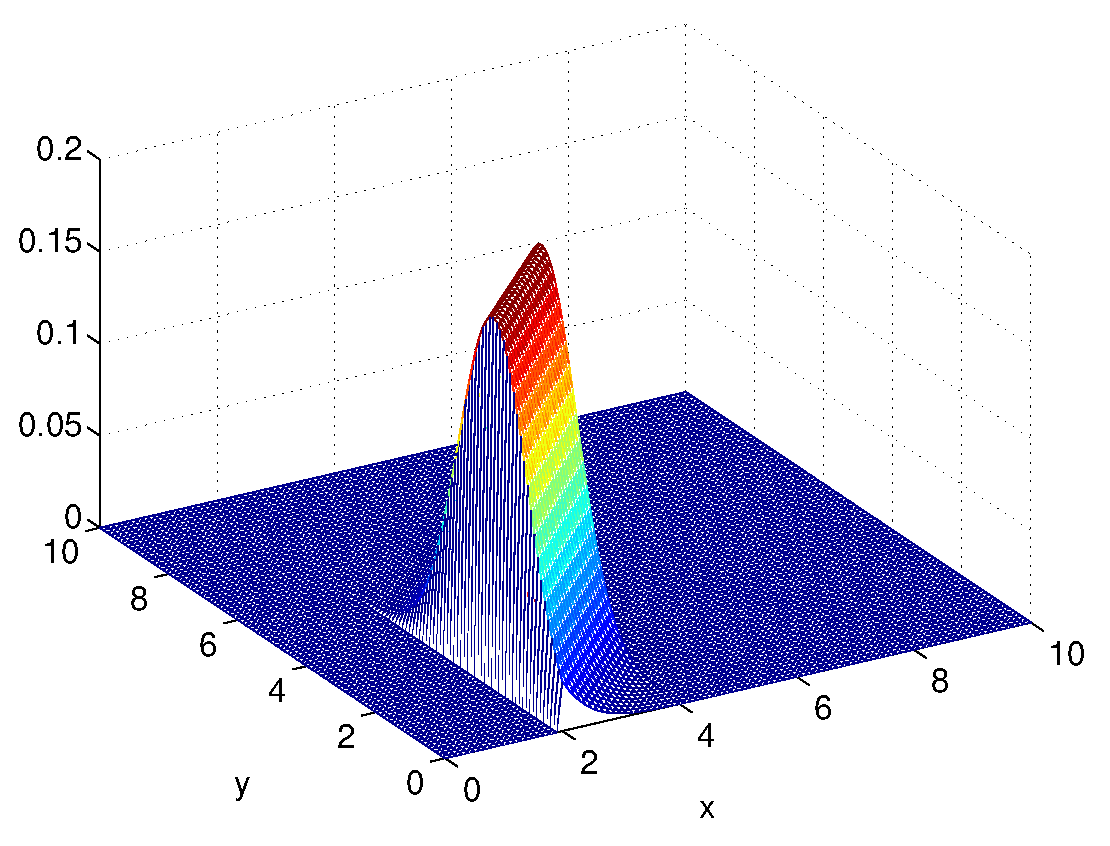
\includegraphics[width=3cm]{./Figures/ProbConjunta.eps} 

\end{column}


\end{columns}

\vspace{-0.3cm}

\color{black} 

\begin{columns}[c]
\begin{column}{5cm}

\visible<2->{
\lstinputlisting{./Matlab/CalculosConjunta.m}}

\end{column}



\begin{column}{5cm}


\visible<3->{
\includegraphics[width=4cm]{./Figures/HistConjunta.eps} }

\vspace{-0.4cm}

\visible<4->{
\lstinputlisting{./Matlab/ResultadosConjunta.m}}

\end{column}
\end{columns}
\end{frame}
\section{Señales aleatorias}
%  %%%%%%%%%%%%%%Empieza la presentacion%%%%%%%%%%%%%%%%%%%%%%%%%%%%%%%%%%

\begin{frame}\frametitle{Señales aleatorias}
  
  \vspace{-0.2cm}
  
  \footnotesize
  
  \begin{itemize}
  \item Una señal aleatoria ($x(t)$ ó $x(n)$) es aquella cuyo comportamiento en cada instante de tiempo ($t$ ó $n$) se encuentra definido por una variable aleatoria asociada al instante de tiempo correspondiente ($X(t)$ ó $X(n)$).
  
  \item Al tener una variable aleatoria asociada a cada instante de tiempo, el comportamiento de la señal a lo largo del tiempo se puede definir
  
  \begin{columns}[c]
  \begin{column}{6cm}
  
  \begin{itemize}
  \footnotesize
  \item Con la función de probabilidad conjunta asociada a todas$^1$ las variables asociadas a la señal aleatoria
  \item A partir de un número infinito de secuencias muestrales.
  \item A partir de los estadísticos relacionados con las variables aleatorias
  \end{itemize}
  
  \end{column}
  \begin{column}{4cm}
  
  
  \color{olivegreen}$p(x(0),x(1),x(2),\dots,x(10))$
  
  \vspace{0.1cm}
  
  \hspace{0.2cm}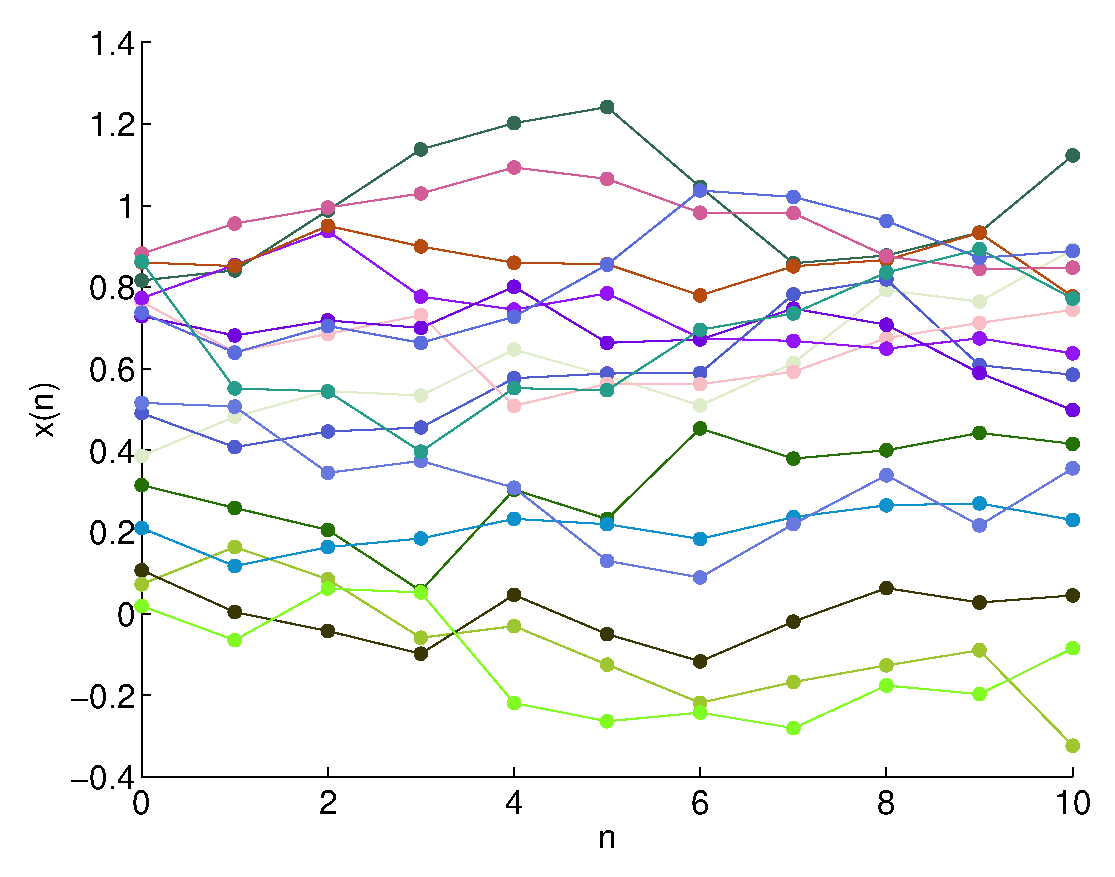
\includegraphics[width=3.5cm]{./Figures/SignalRandomDisc.eps}
  
  Ejemplos: $\mu_{x(n)}$, $\phi_{x(n)x(m)}$
  
  
  \end{column}
  \end{columns}
  
  
  \end{itemize}
  
  \rule{11cm}{0.04ex}
  \scriptsize
  
  $^1$ En principio, si la variable independiente es continua tendremos infinitas variables aleatorias, mientras que si la variable independiente es discreta tendremos tantas variables aleatorias como instantes de $n$ estemos analizando.
  
\end{frame}
  
  
  
\begin{frame}
\frametitle{Señales aleatorias}

\vspace{-0.2cm}

\footnotesize

\begin{itemize}
\item Una señal aleatoria ($x(t)$ ó $x(n)$) es aquella cuyo comportamiento en cada instante de tiempo ($t$ ó $n$) se encuentra definido por una variable aleatoria asociada al instante de tiempo correspondiente ($X(t)$ ó $X(n)$).

\item Al tener una variable aleatoria asociada a cada instante de tiempo, el comportamiento de la señal a lo largo del tiempo se puede definir

\begin{columns}[c]
\begin{column}{6cm}

\begin{itemize}
\footnotesize
\item Con la función de probabilidad conjunta asociada a todas$^1$ las variables asociadas a la señal aleatoria
\item A partir de un número infinito de secuencias muestrales.
\item A partir de los estadísticos relacionados con las variables aleatorias
\end{itemize}

\end{column}
\begin{column}{4cm}


\color{olivegreen}$p(x(0),x(1),x(2),\dots,x(10))$

\vspace{0.1cm}

\hspace{0.2cm}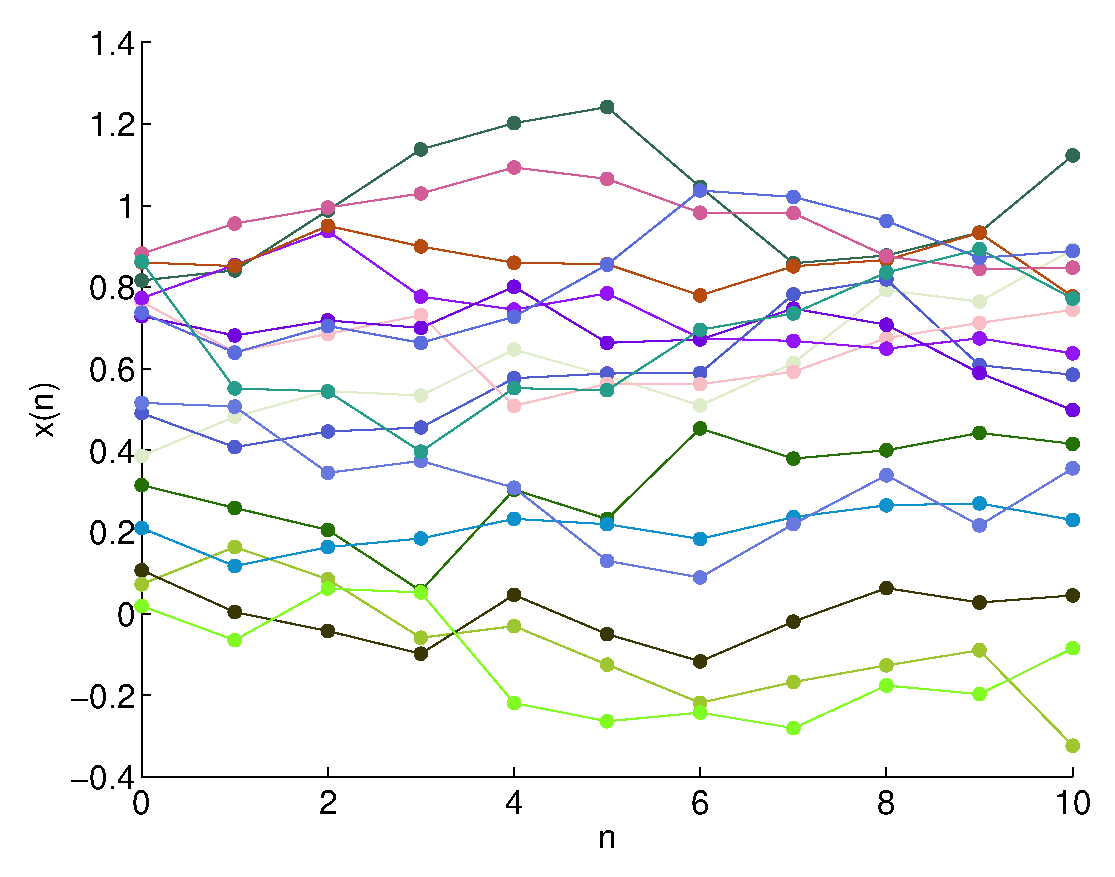
\includegraphics[width=3.5cm]{./Figures/SignalRandomDisc.eps}

Ejemplos: $\mu_{x(n)}$, $\phi_{x(n)x(m)}$


\end{column}
\end{columns}


\end{itemize}

\rule{11cm}{0.04ex}
\scriptsize

$^1$ En principio, si la variable independiente es continua tendremos infinitas variables aleatorias, mientras que si la variable independiente es discreta tendremos tantas variables aleatorias como instantes de $n$ estemos analizando.

\end{frame}

%%%%%%%%%%%%%%%%%%%%%%%%%%%%%%%%%%%%%%%%%%%%%%%%


\begin{frame}
\frametitle{Estadísticos de las señales aleatorias}

\vspace{-0.2cm}

\footnotesize

\begin{itemize}

\item Los estadísticos de una señal aleatoria, o de un par de señales aleatorias, se calculan de la misma forma que se calcula los estadísticos de conjuntos de variables aleatorias:
\begin{itemize}
\footnotesize
\item Probabilidades necesarias:

\begin{itemize}

\scriptsize

\item La probabilidad de la señal en cada instante: $p_{X(t)}(x(t))\triangleq p_X(x,t)$.

\item La probabilidad conjunta:

\hspace{0.2cm}De 1 señal en 2 instantes: $p_{X(t_1)X(t_2)}(x(t_1),x(t_2))\triangleq p_X(x_1,t_1,x_2,t_2)$.

\hspace{0.2cm}De 2 señales en 2 instantes: $p_{X_i(t_i)X_j(t_j)}(x_i(t_i),\!x_j(t_j))\!\triangleq \! p_{X_iX_j}(x_i,\!t_i,\!x_j,\!t_j)$.

\end{itemize}

\item Estadísticos habituales:

\begin{itemize}

\scriptsize

\item  Media: $\mu_X(t)\triangleq \mu_{X(t)}=\int_{-\infty}^\infty x(t)p(x(t))dx(t)=\int_{-\infty}^\infty xp(x,t)dx$

\item  Valor cuadrático medio: $\Psi_X(t)\triangleq  E(X^2(t))=\int_{-\infty}^\infty x^2(t)p(x(t))dx(t)=\int_{-\infty}^\infty x^2p(x,t)dx$

\item  Correlación cruzada: $\phi_{X_i,X_j}(t_i,t_j) \triangleq \phi_{X_i(t_i),X_j(t_j)}=\int_{-\infty}^\infty x_i(t_i)x_j(t_j)p(x_i(t_i),x_j(t_j))dx_i(t_i)dx_j(t_j)=\int_{-\infty}^\infty x_ix_jp(x_i,t_i,x_j,t_j)dx_idx_j$

\item Autocorrelación: $\phi_{XX}(t_1,t_2) \triangleq \phi_{X(t_1),X(t_2)}=\int_{-\infty}^\infty x(t_1)x(t_2)p(x(t_1),x(t_2))dx(t_1)dx(t_2)=\int_{-\infty}^\infty x_1x_2p(x_1,t_1,x_2,t_2)dx_1dx_2$

\end{itemize}

\end{itemize}
\end{itemize}


\rule{11cm}{0.04ex}
\scriptsize

Estas probabilidades se podrían obtener marginalizando de las conjuntas de la secuencia de la señal o de las secuencias de las señales las variables que no están involucradas en la probabilidad final.


\end{frame}


%%%%%%%%%%%%%%%%%%%%%%%%%%%%%%%%%%%%%%%%%%%%%%%%%


\begin{frame}
\frametitle{Tipos de señales aleatorias I}

\vspace{-0.2cm}

\footnotesize

\begin{itemize}
\item \alert{Señal Markoviana Discreta de Orden I: }

\begin{itemize}
\footnotesize
\item La probabilidad de la señal en un instante únicamente depende del valor de la variable en el instante anterior:  $p(x(n)|x(n-1))$

\vspace{0.1cm}

\visible<2->{

\item Este hecho permite realizar una factorización muy conveniente:
{\scriptsize

\vspace{0.1cm}

$p(x(0),x(1),\cdots,x(n))=$

\vspace{0.1cm}

\hspace{0.3cm}$=p(x(0)p(x(1)|x(0))p(x(2)|x(0),x(1))\cdots p(x(n)|x(0),\cdots,x(n-1))=$

\vspace{0.1cm}

\hspace{0.3cm}$=p(x(0))p(x(1)|x(0))p(x(2)|x(1))\cdots p(x(n)|x(n-1))=$

\vspace{0.1cm}

\hspace{0.3cm}$=p(x(0))\prod_{i=1}^n p(x(n)|x(n-1))$

}}
\end{itemize}


\end{itemize}



\visible<3->{

\color{olivegreen}Ejemplo: random walk gaussiano \color{gray}

\vspace{0.1cm}

{\scriptsize

\hspace{0.3cm}$p(x(0))=\mathcal{N}_X(x(0);1;0.1)$

\vspace{0.1cm}

\hspace{0.3cm}$p(x(n)|x(n-1))=\mathcal{N}_X(x(n);x(n-1);0.25)$ \visible<4->{$\rightarrow x(n)=x(n-1)+sqrt(0.25)*randn$}


}


\begin{columns}[c]
\begin{column}{6cm}

\vspace{-0.4cm}
\visible<5->{
\lstinputlisting{./Matlab/ProcMarkov.m}
}
\end{column}
\begin{column}{4cm}

\visible<6->{
\vspace{0.2cm}
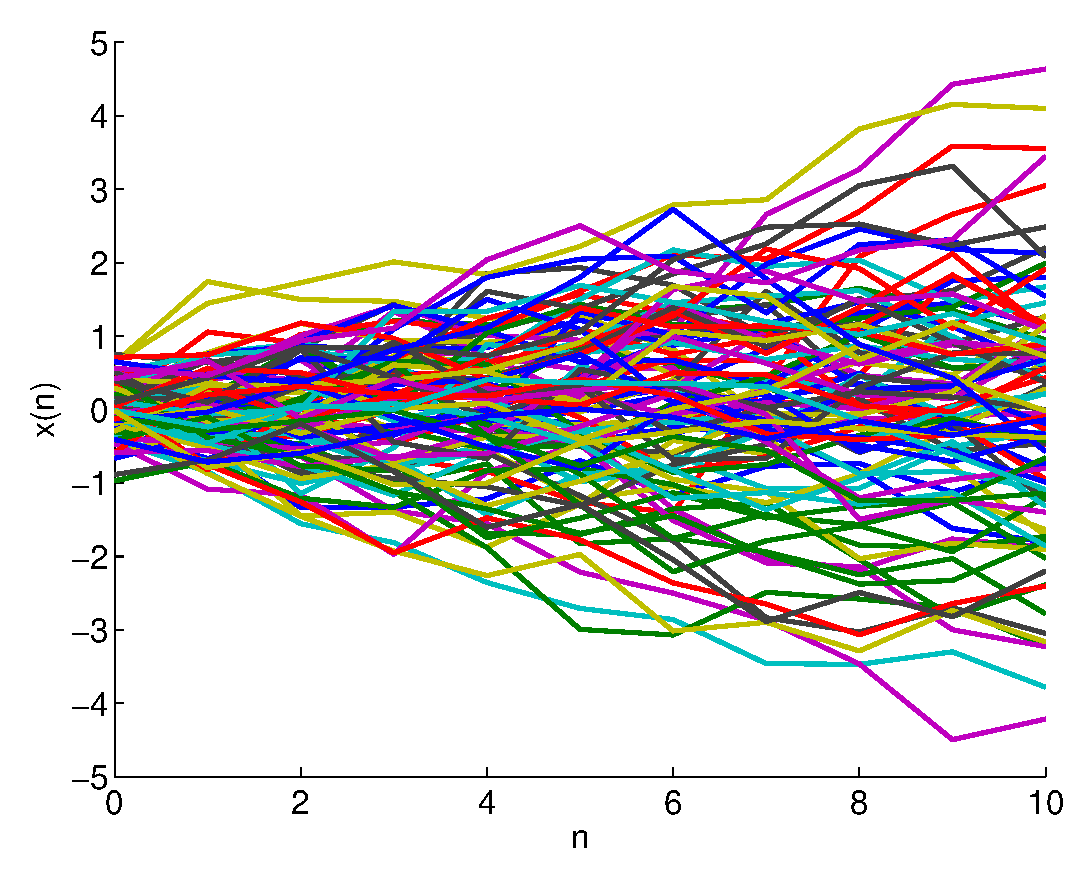
\includegraphics[width=3.5cm]{./Figures/RandomWalk.eps}
}
\end{column}
\end{columns}
}

\end{frame}

%%%%%%%%%%%%%%%%%%%%%%%%%%%%%%%%%%%%%%%%%%%%%%

\begin{frame}
\frametitle{Tipos de señales aleatorias II}


\footnotesize

\begin{itemize}
\item \alert{Señal Markoviana Continua de Orden I: }

\begin{itemize}
\footnotesize

\item Mientras que a la hora de modelar sistemas/señales discretos se utilizan los retardos para relacionar las variables, a la hora de modelar sistemas/señales continuos se utilizan las derivadas:

\vspace{0.1cm}
{
\color{olivegreen}
\hspace{0.5cm}Ejemplo discreto: $y(k)+y(k-1)+y(k-2)=x(k)$

\vspace{0.1cm}

\hspace{0.5cm}Ejemplo continuo: $\ddot y(t)+ \dot y(t) +y(t)=x(t)$

\vspace{0.1cm}

\color{black}}

\visible<2->{

\item Por lo tanto, la relación probabilística que se establece en señales Markovianas discretas entre una señal y su versión retardada, en señales Markovianas continuas se establece entre la derivada de la señal y la señal sin derivar:
  $p(\dot x(t)|x(t))$
}


\visible<3->{

\hspace{0.5cm}\color{olivegreen}Ejemplo: proceso Markov gaussiano \color{gray}

\vspace{0.1cm}




\scriptsize

\hspace{0.8cm}$p(x(0))=\mathcal{N}_X(x(0);1;0.1)$

\vspace{0.1cm}

\hspace{0.8cm}$p(\dot x(t)|x(t))\!=\!\mathcal{N}_X(\dot x(t);x(t);0.25)$

\vspace{0.1cm}

 \hspace{3.8cm}$\rightarrow \dot x(t)\!=\!x(t)\!+\!u(t)$ con $u(t)=\mathcal{N}_{U}(u,0,1)$

\hspace{0.8cm}Lo podríamos simular con lsim o Simulink, suponiendo un sistema de primer orden.

}

\end{itemize}
\end{itemize}

\end{frame}

%%%%%%%%%%%%%%%%%%%%%%%%%%%%%%%%%%%%%%%%%%%%%%

\begin{frame}
\frametitle{Tipos de señales aleatorias III}

\vspace{-0.2cm}

\footnotesize

\begin{itemize}
\item \alert{Señales aleatorias estacionarias (en sentido amplio): }
\begin{itemize}
\footnotesize

\visible<2->{
\item Son aquellas señales en las que la función de probabilidad no depende del tiempo: $p(x(t_1))=p(x(t_2))\triangleq p(x)$}

\vspace{0.1cm}

\visible<3->{

\item Este hecho implica que:

}

\begin{itemize}

\visible<3->{

\item Los estadísticos de una variable no dependen del tiempo:

\scriptsize

\vspace{0.1cm}

\hspace{0.2cm}Media: $\mu_X(t)\triangleq\int_{-\infty}^\infty x(t)p(x(t))dx(t)=\int_{-\infty}^\infty xp(x)dx= \alert{\mu_X}$


\vspace{0.1cm}

\hspace{0.2cm}Valor cuadrático medio:

\vspace{0.1cm}

\hspace{0.2cm}$\Psi_X(t)=\int_{-\infty}^\infty x^2(t)p(x(t))dx(t)=\int_{-\infty}^\infty x^2p(x)dx=\alert{\Psi_X}$

\vspace{0.1cm}

\hspace{0.2cm}Varianza: $\sigma^2_X(t)=\Psi_X(t)-\mu^2_X(t)=\Psi_X-\mu^2_X=\alert{\sigma^2_X}$


}

\vspace{0.1cm}

\visible<4->{
\footnotesize

\item Los estadísticos de dos variables dependen de la diferencia temporal:

\scriptsize

\vspace{0.1cm}

\hspace{0.2cm}Correlación cruzada:


\hspace{0.3cm}$\phi_{X_i,X_j}(t_i,t_j) =\int_{-\infty}^\infty x_i(t_i)x_j(t_j)p(x_i(t_i),x_j(t_j))dx_i(t_i)dx_j(t_j)=$

\hspace{0.4cm}$\int_{-\infty}^\infty x_i(t)x_j(t+\tau)p(x_i(t),x_j(t+\tau))dx_i(t)dx_j(t+\tau)=\alert{\phi_{X_iX_j}(\tau)}$

\vspace{0.1cm}

\hspace{0.2cm}Autocorrelación:

\hspace{0.3cm}$\phi_{XX}(t_1,t_2) =\int_{-\infty}^\infty x(t_1)x(t_2)p(x(t_1),x(t_2))dx(t_1)dx(t_2)=$

\hspace{0.4cm}$\int_{-\infty}^\infty x(t)x(t+\tau)p(x(t),x(t+\tau))dx(t)dx(t+\tau)=\alert{\phi_{XX}(\tau)}$
}
\end{itemize}

\end{itemize}
\end{itemize}
\end{frame}
%%%%%%%%%%%%%%%%%%%
\begin{frame}
\frametitle{Tipos de señales aleatorias IV}

\footnotesize

\vspace{-0.1cm}

\color{olivegreen}¿Cuales de las señales siguientes son estacionarias (en sentido amplio)?





%%%%%%%%%%%%%%%%%%%%%%%%

\begin{columns}[T]
\hspace{-0.5cm}\begin{column}{7cm}

\color{olivegreen}Ej1: ¿sistema discreto con variables $x(n)$ independientes y $p(x(n))=\mathcal{U}_{[a,b]}(x(n))$


 \color{gray}


\visible<2->{
\vspace{0.0cm}

Si, ya que las variables son independientes y tienen la misma función de probabilidad a lo largo del tiempo.
}
\end{column}
\begin{column}{2.5cm}
\visible<2->{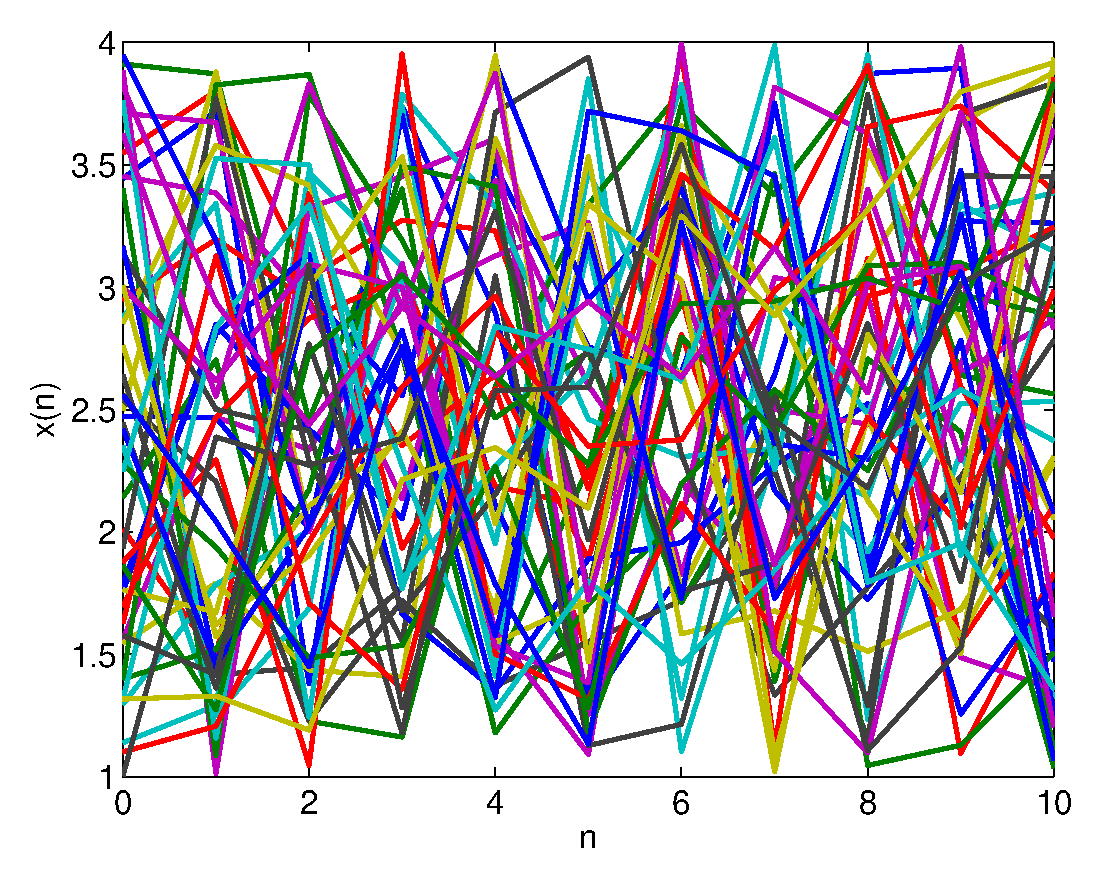
\includegraphics[width=2cm]{./Figures/Est1.eps}}
\end{column}
\end{columns}



%%%%%%%%%%%%%%%%%%%%%%%%%

\vspace{0.2cm}

\visible<3->{
\begin{columns}[T]
\hspace{-0.5cm}\begin{column}{7cm}




\color{olivegreen}Ej2: ¿sistema discreto con variables $x(n)$ independientes y $p(x(n))=\mathcal{N}_X(x(n);\mu_x,(0.5)^{n})$


 \color{gray}


\visible<4->{
\vspace{0.1cm}

No, ya que aunque las variables son independientes la función de probabilidad cambia a lo largo del tiempo.
}
\end{column}
\begin{column}{2.5cm}
\visible<4->{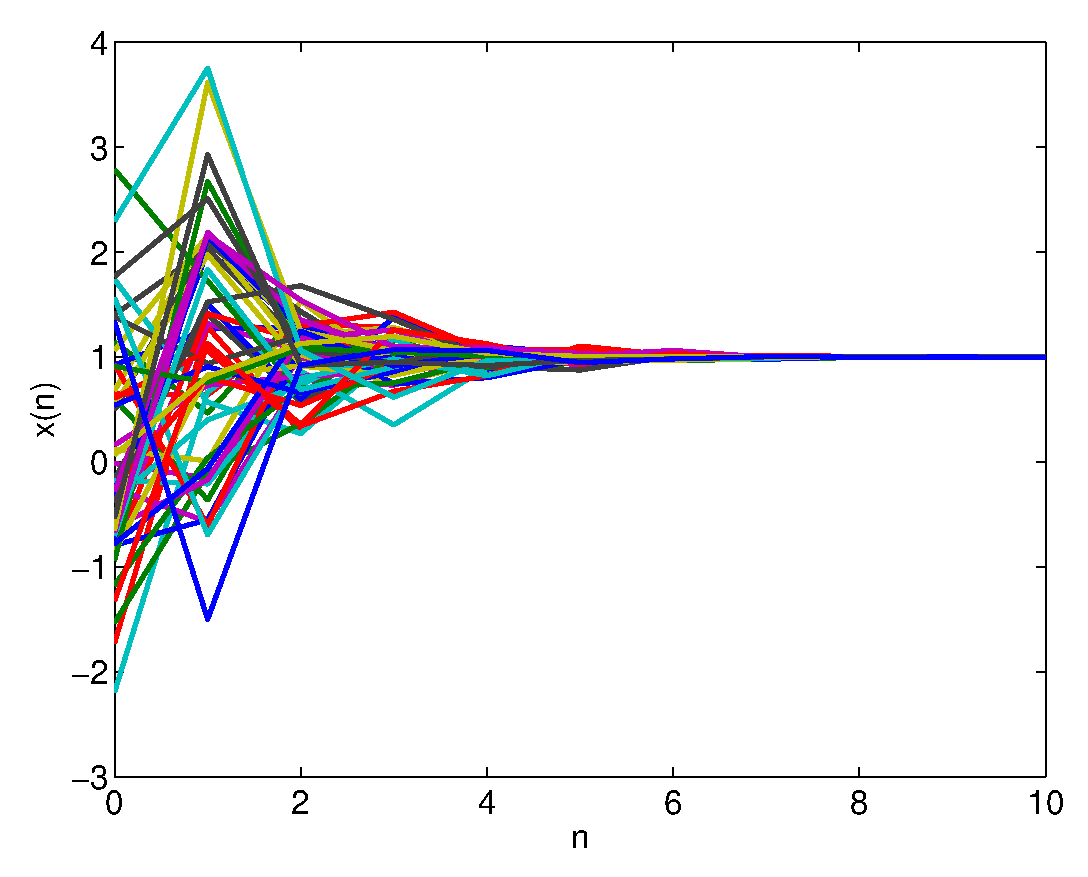
\includegraphics[width=2cm]{./Figures/Est2.eps} }
\end{column}
\end{columns}
}

%%%%%%%%%%%%%%%%%%%%%%%%%%%%%%%%%


\vspace{0.3cm}

\visible<5->{
\begin{columns}[T]
\hspace{-0.5cm}\begin{column}{7cm}

\color{olivegreen}Ej3: ¿random walk gaussiano discreto propuesto? \color{gray}


\visible<6->{
\vspace{-0.3cm}

No, ya que la varianza del proceso (estadístico de una variable) aumenta a lo largo del tiempo.
}
\end{column}
\begin{column}{2.5cm}
\visible<5->{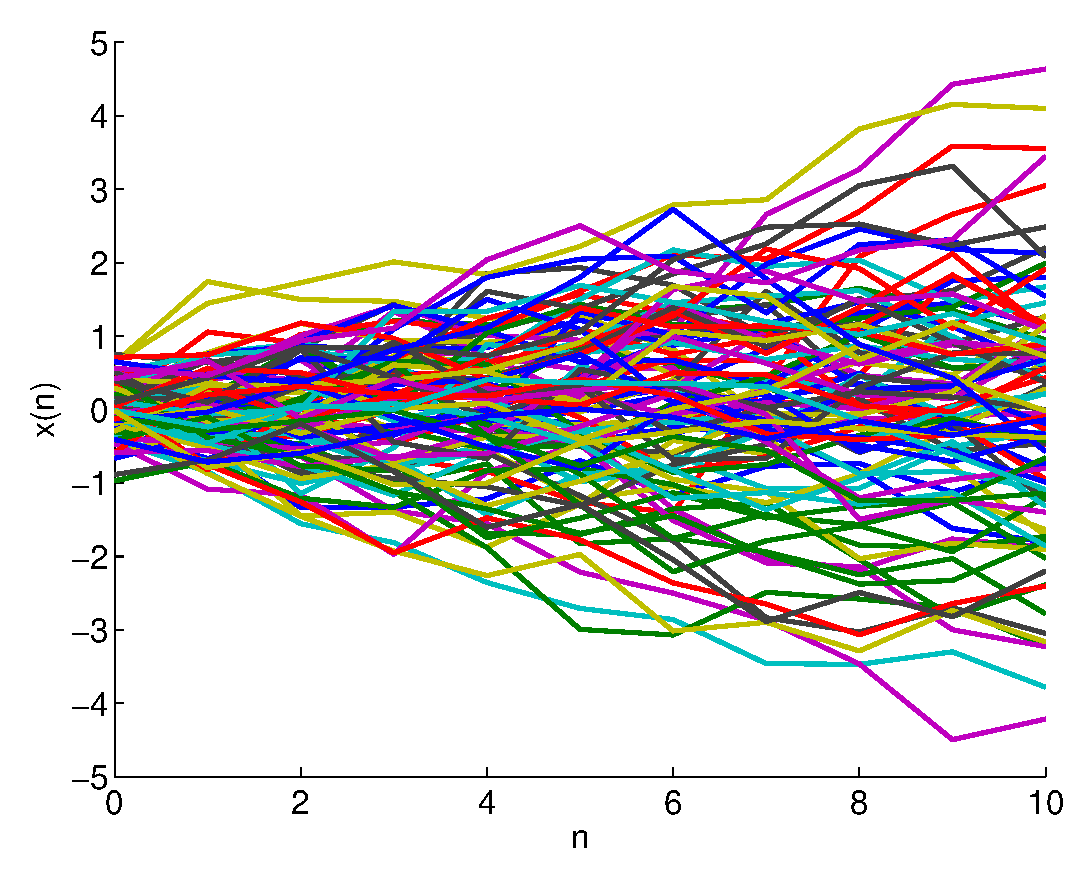
\includegraphics[width=2cm]{./Figures/RandomWalk.eps}}
\end{column}
\end{columns}

}

\vspace{0.1cm}

\visible<7->{
\begin{columns}[T]
\hspace{-0.5cm}\begin{column}{7cm}

\color{olivegreen}Ej4: Markoviano discreto $p(x(0))=U_{[a,b]}(x(0))$ y $p(x(n)|x(n-1))=\delta(x(n)-x(n-1))$  \color{gray}


\visible<8->{
\vspace{0.0cm}

Si, ya que se puede demostrar que $p(x(n))=U_{[a,b]}(x(n))$.
}
\end{column}
\begin{column}{2.5cm}
\visible<6->{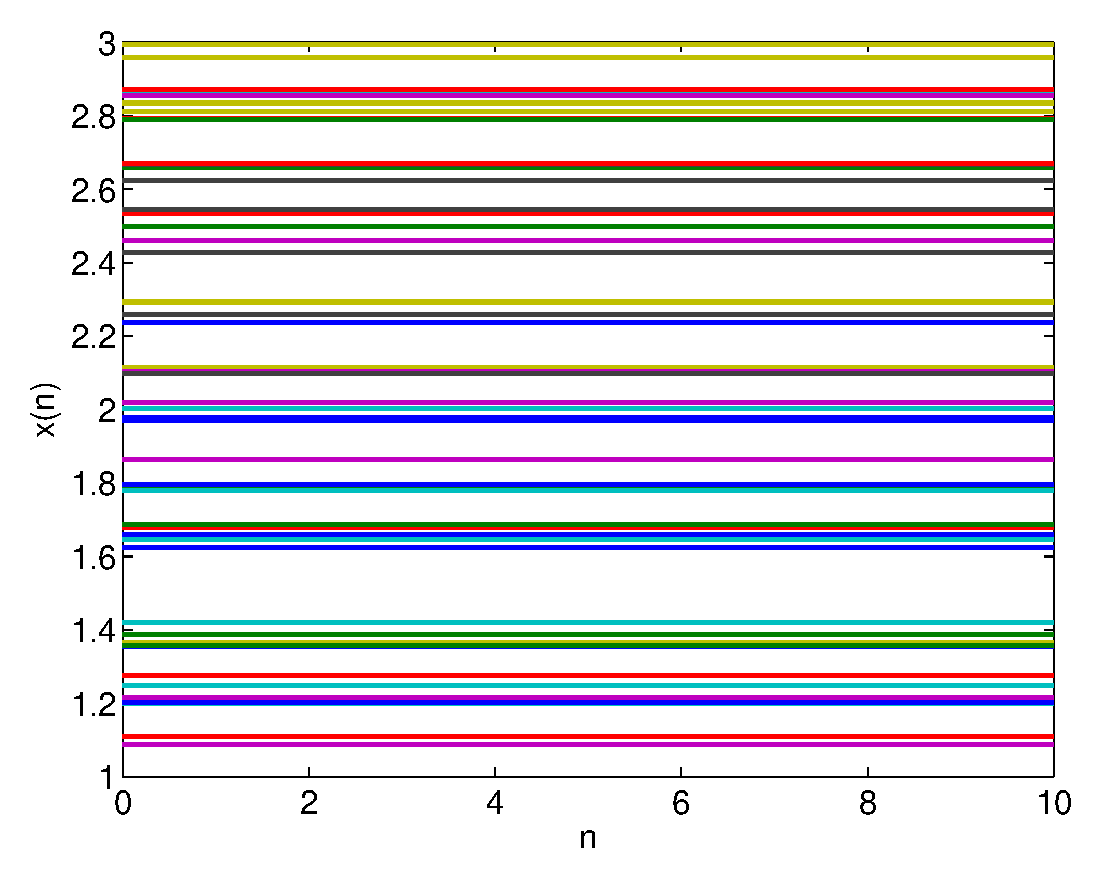
\includegraphics[width=2cm]{./Figures/Est3.eps}}
\end{column}
\end{columns}

}


\end{frame}

%%%%%%%%%%%%%%%%%%%%%%%%%%%%%%%%%%%%%%%%%%


\begin{frame}
\frametitle{Tipos de señales aleatorias V}

\vspace{-0.2cm}

\footnotesize

\begin{itemize}
\item \alert{Señales ergódicas: }
\begin{itemize}
\footnotesize
\item Son señales aleatorias \alert{estacionarias} cuyos estadísticos pueden ser caracterizados directamente a partir de una muestra (secuencia de valores) de la señal.

\visible<2->{
\item Es decir, en vez de tener que utilizar la función de probabilidad conjunta o las infinitas muestras de la señal en cada  instante de tiempo, los estadísticos se pueden estimar a partir de los valores de una muestra de la señal real.
}

\visible<3->{
\item La redefinición de los estadísticos a partir de una muestra (secuencia de valores) de la señal no requiere de funciones de probabilidad, si no del cálculo de la media, ... y correlación de las señales directamente:

\begin{itemize}
\scriptsize

\item Media: $\mu_X \triangleq \lim_{T \rightarrow \infty} \frac{1}{2T}\int_{-T}^T x(t)dt$


\vspace{0.1cm}

\item Valor cuadrático medio: $\Psi_X \triangleq \lim_{T \rightarrow \infty} \frac{1}{2T} \int_{-T}^T x^2(t)dt$


\vspace{0.1cm}

\item Correlación cruzada: $\phi_{X_i,X_j}(\tau)  \triangleq \lim_{T \rightarrow \infty} \frac{1}{2T}\int_{-T}^T x_i(t)x_j(t+\tau)dt$

\item Autocorrelación: $\phi_{XX}(\tau) \triangleq \lim_{T \rightarrow \infty} \frac{1}{2T}\int_{-T}^T x(t)x(t+\tau)dt$

\end{itemize}
}

\end{itemize}
\end{itemize}

\end{frame}

%%%%%%%%%%%%%%%%%%%%%%%%%

%%%%%%%%%%%%%%%%%%%%%%%%%%%%%%%%%%%%%%%%%%


\begin{frame}
\frametitle{Tipos de señales aleatorias VI}

\footnotesize

\vspace{-0.1cm}

\color{olivegreen}¿Cuales de las señales siguientes son ergódicas?





%%%%%%%%%%%%%%%%%%%%%%%%

\begin{columns}[T]
\hspace{-0.5cm}\begin{column}{7cm}

\color{olivegreen}Ej1: ¿sistema discreto con variables $x(n)$ independientes y $p(x(n))=\mathcal{U}_{[a,b]}(x(n))$


 \color{gray}


\visible<2->{
\vspace{0.0cm}

Si, ya que es estacionario y se puede obtener los estadísticos de una única secuencia de valores.
}
\end{column}
\begin{column}{2.5cm}
\visible<2->{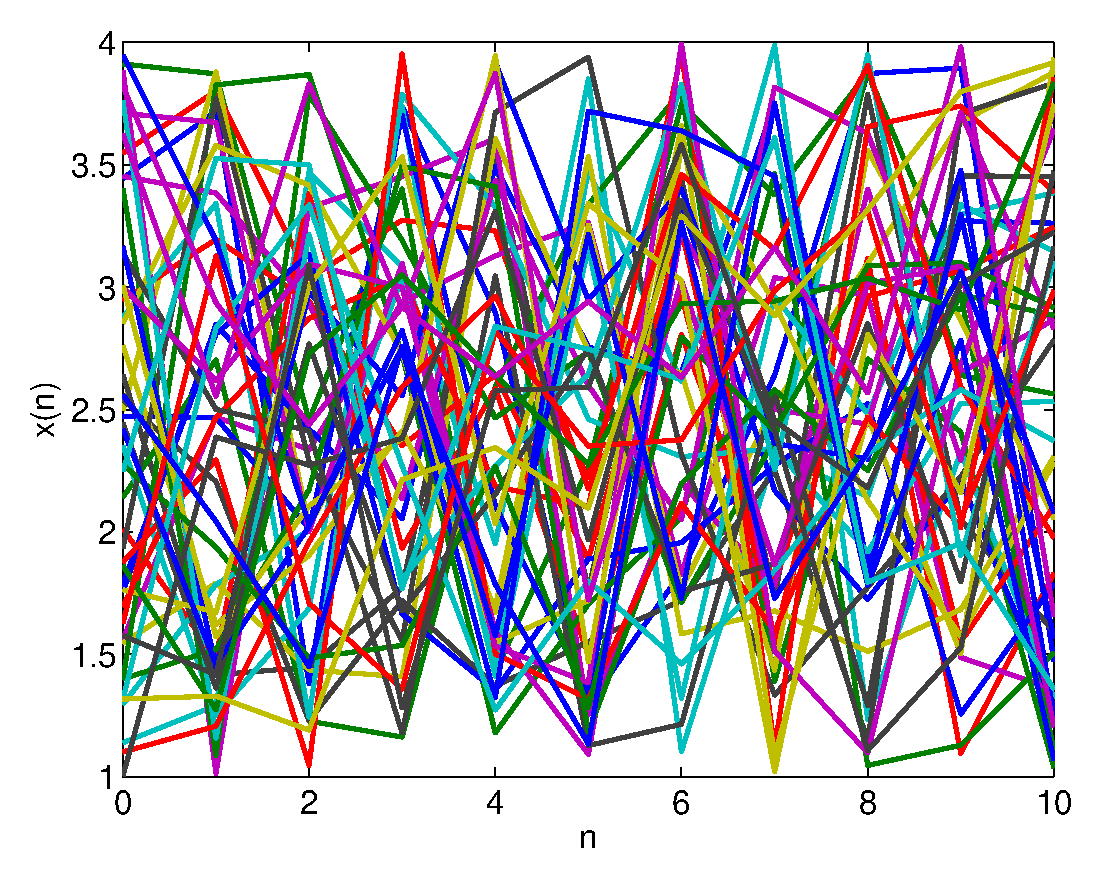
\includegraphics[width=2cm]{./Figures/Est1.eps}}
\end{column}
\end{columns}



%%%%%%%%%%%%%%%%%%%%%%%%%

\vspace{0.2cm}

\visible<3->{
\begin{columns}[T]
\hspace{-0.5cm}\begin{column}{7cm}




\color{olivegreen}Ej2: ¿sistema discreto con variables $x(n)$ independientes y $p(x(n))=\mathcal{N}_X(x(n);\mu_x,(0.5)^{n})$


 \color{gray}


\visible<4->{
\vspace{0.1cm}

No, ya que no es estacionario.
}
\end{column}
\begin{column}{2.5cm}
\visible<4->{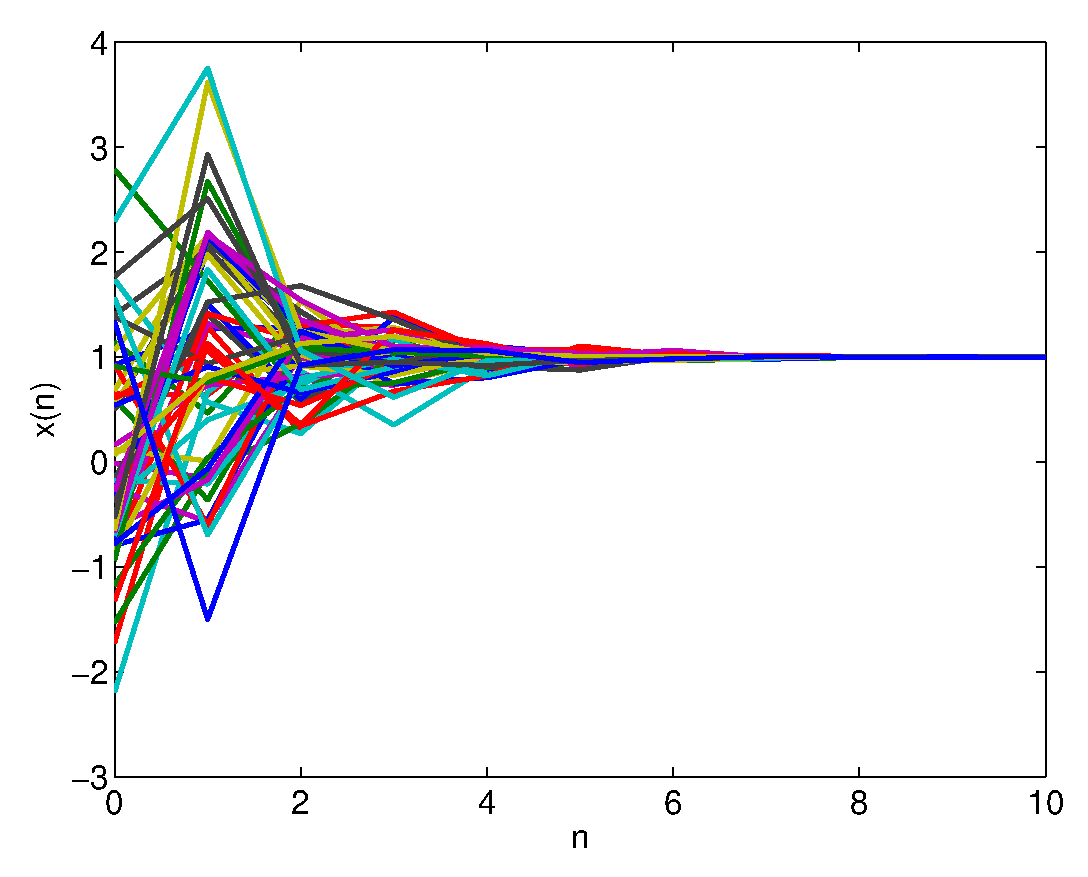
\includegraphics[width=2cm]{./Figures/Est2.eps} }
\end{column}
\end{columns}
}

%%%%%%%%%%%%%%%%%%%%%%%%%%%%%%%%%


\vspace{0.3cm}

\visible<5->{
\begin{columns}[T]
\hspace{-0.5cm}\begin{column}{7cm}

\color{olivegreen}Ej3: ¿random walk gaussiano discreto propuesto? \color{gray}


\visible<6->{
\vspace{-0.3cm}

No, ya que no es estacionario.
}
\end{column}
\begin{column}{2.5cm}
\visible<5->{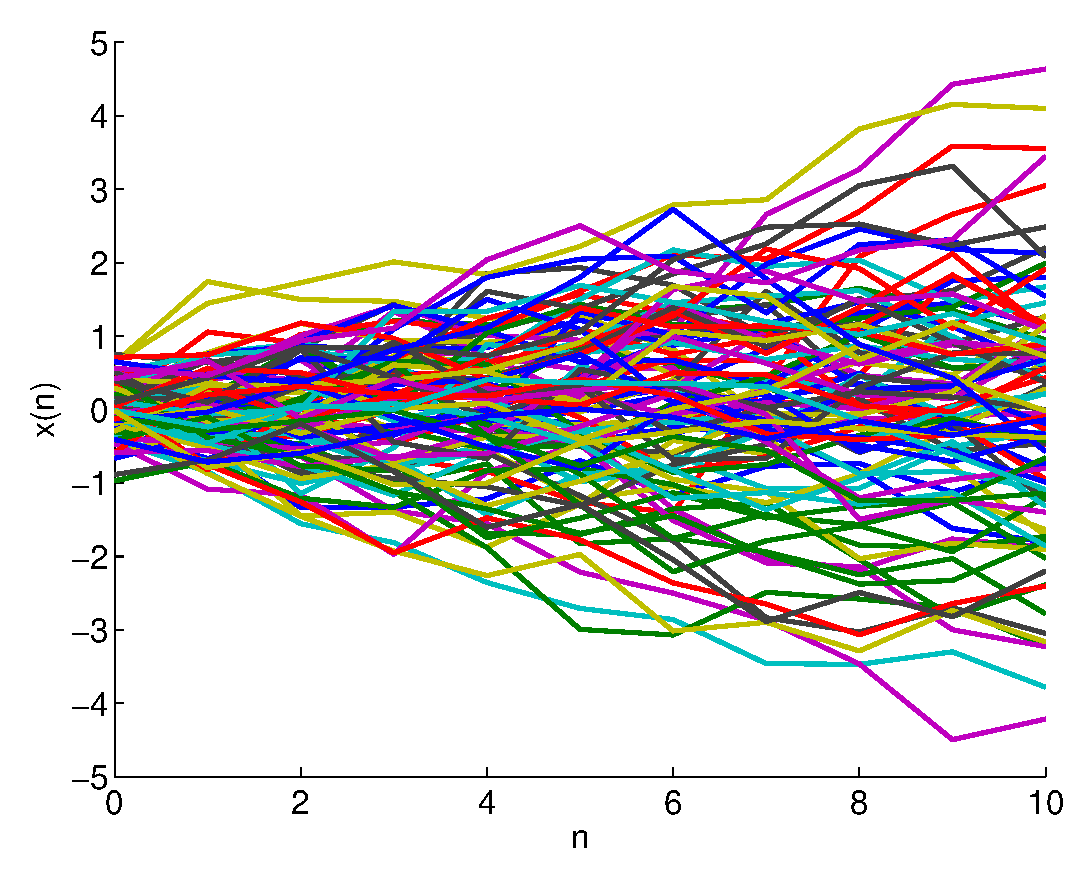
\includegraphics[width=2cm]{./Figures/RandomWalk.eps}}
\end{column}
\end{columns}

}

\vspace{0.1cm}

\visible<7->{
\begin{columns}[T]
\hspace{-0.5cm}\begin{column}{7cm}

\color{olivegreen}Ej4: Markoviano discreto $p(x(0))=U_{[a,b]}(x(0))$ y $p(x(n)|x(n-1))=\delta(x(n)-x(n-1))$  \color{gray}


\visible<8->{
\vspace{0.0cm}

No, ya que una secuencia de valores no es representativa de la muestra (cada señal toma un valor constante).
}
\end{column}
\begin{column}{2.5cm}
\visible<6->{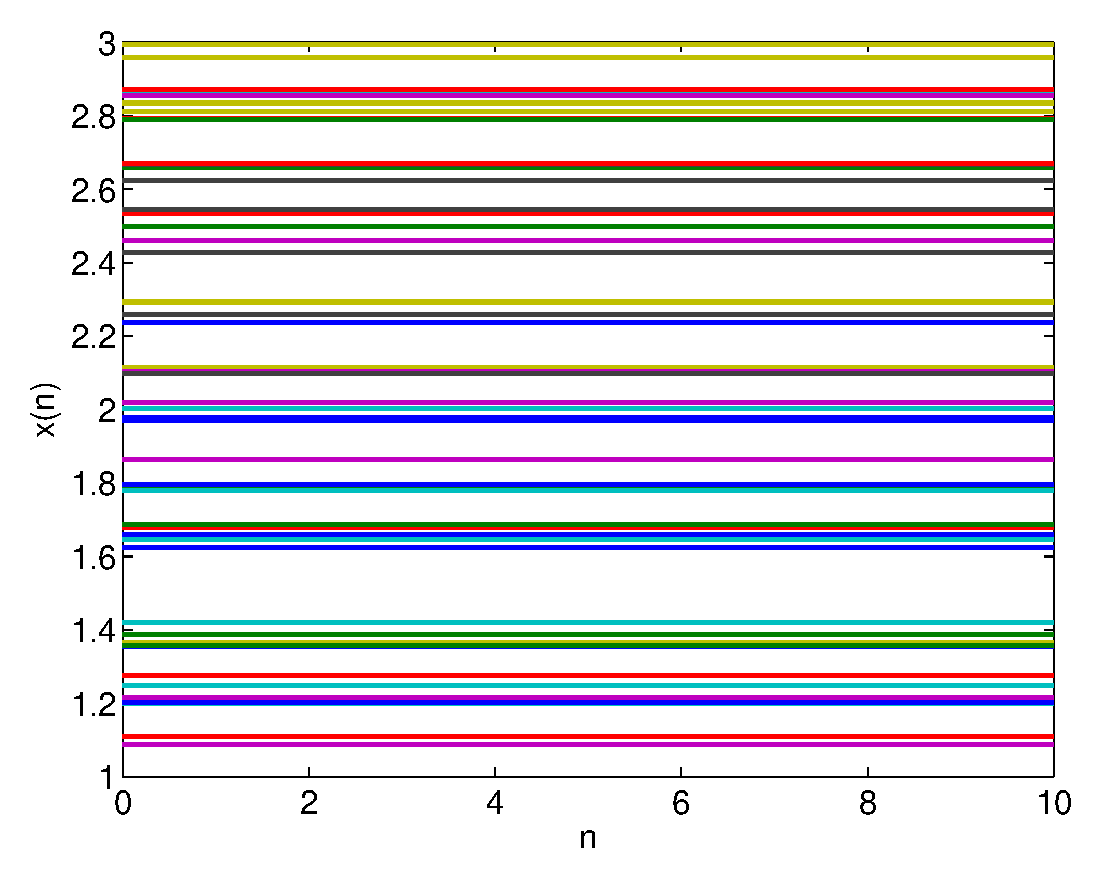
\includegraphics[width=2cm]{./Figures/Est3.eps}}
\end{column}
\end{columns}

}

\end{frame}





%%%%%%%%%%%%%%%%%%%%%%



\begin{frame}
\frametitle{Señales aleatorias estacionarias: Propiedades I}

\footnotesize

\begin{itemize}

\item Media ($\mu_X$), Valor cuadrático medio ($\Psi_X$), y la varianza $\sigma_X^2$ son constantes en el tiempo.
\item Correlación cruzada ($\phi_{XY}(\tau)$), autocorrelacion ($\phi_{XX}(\tau)$) y covarianza cruzada ($\phi_{XY}(\tau)$) dependen de la diferencia temporal $\tau$.

\item Relaciones con la autocorrelación:


\begin{itemize}

\footnotesize

\item La autocorrelación en el instante inicial es igual al valor cuadrático medio: $\phi_{XX}(0)=\Psi_X=E(X^2)$.

{\scriptsize
\color{gray}

$\Psi_X=E(X^2)=\int x^2(t) p(x(t))dx(t)$

$\phi_{XX}(\tau)=\int x(t)x(t+\tau) p(x(t),x(t+\tau))dx(t)$
}

\item $\phi_{XX}(\infty)=|\mu_X|^2.$

\item $\phi_{XX}(0)>\phi_{XX}(\tau)$  (el máximo de la autocorrelación está en cero)

\item Estas propiedades nos pueden permitir saber si la señal tiene una componente determinista o no:

\begin{itemize}

\item Si no la tiene deberá tender al valor medio según pasa el tiempo.
\item Si la tiene  la autocorrelación tendrá un comportamiento diferente.
\item Aun más, en el caso en que la señal tenga un comportamiento determinista periódico, la autocorrelación también mostrará el comportamiento periódico.
\end{itemize}
\end{itemize}
\end{itemize}


\end{frame}

%%%%%%%%%%%%%%%%%%%%%%%%%%%%%%%%%%%%%%%%%%%%%%%

\begin{frame}
\frametitle{Señales aleatorias estacionarias: Propiedades II}

\footnotesize

\vspace{-0.1cm}

\color{olivegreen}Ejemplos de autocorrelación de señales ergódicas (usadas como casos de estacionarias porque permiten cálculos a partir de una secuencia de valores).

\begin{itemize}

\scriptsize
\item \color{blue}\texttt{[phixy,lags]=xcorr(x,y,limk,'unbiased')}: \color{black}cálculo de la correlación$^1$ cruzada de las señales x e y.
\item \color{blue}\texttt{[phixy,lags]=xcorr(x,limk,'unbiased')}: \color{black} cálculo de la autocorrelación$^1$ de la señal x.

\end{itemize}

%%%%%%%%%%%%%%%%%%%%%%%%

\visible<2->{

\begin{columns}[T]
\hspace{-0.5cm}\begin{column}{6cm}

\color{olivegreen}Ej1: Sistema continuo con variables $x(t)$ independientes y $p(x(t))=\mathcal{N}(x(t);5,1)$

\color{black}

\vspace{0.1cm}

Lo discretizamos con periodo $T_s=0.01$

\vspace{-0.3cm}

\lstinputlisting{./Matlab/Auto1.m}

\end{column}
\begin{column}{4cm}
\visible<3->{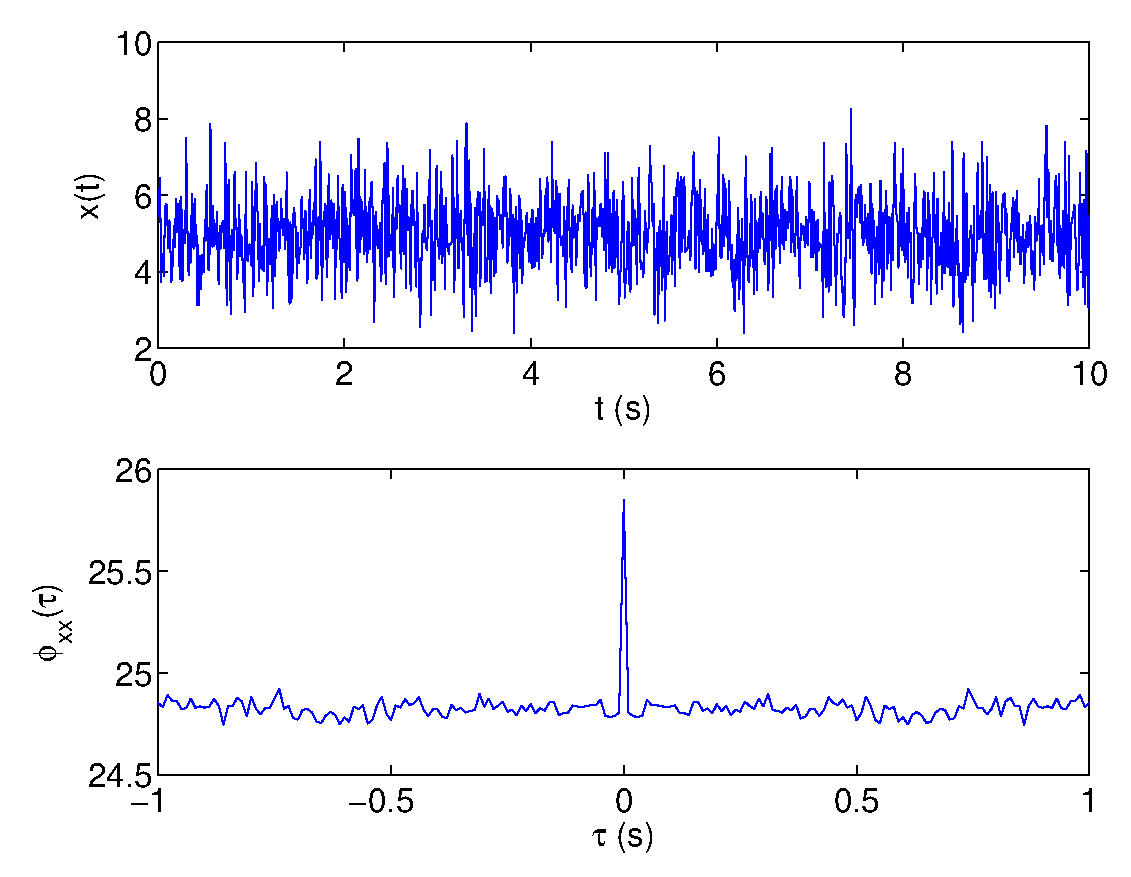
\includegraphics[width=3.2cm]{./Figures/Auto1.eps}

\scriptsize
\color{gray}
$\phi_{XX}(0)=\Psi_X=\sigma^2_X+\mu^2_X=26$

$\phi_{XX}(\infty) \rightarrow \mu^2_X=25$}



\end{column}
\end{columns}

}

\rule{11cm}{0.04ex}
\scriptsize

$^1$\color{blue}\texttt{liml } \color{black} se utiliza para limitar los valores de la $k$ sobre los que se calcula la correlación y la autocorrelación. Los límites temporales están $\tau=\pm T_s limk$.

\end{frame}

%%%%%%%%%%%%%%%%%%%%%%%%%

\begin{frame}

\frametitle{Señales aleatorias estacionarias: Propiedades III}

\footnotesize

\vspace{-0.1cm}

\begin{columns}[T]
\hspace{-0.5cm}\begin{column}{6cm}

\color{olivegreen}Ej2: Sistema continuo con variables $x(t)$ independientes y $p(x(t))=\mathcal{U}_{[2,6]}(x(t))$

\color{black}

\vspace{0.1cm}

Lo discretizamos con periodo $T_s=0.01$


\vspace{-0.3cm}

\lstinputlisting{./Matlab/Auto2.m}

\end{column}
\begin{column}{4cm}
\visible<2->{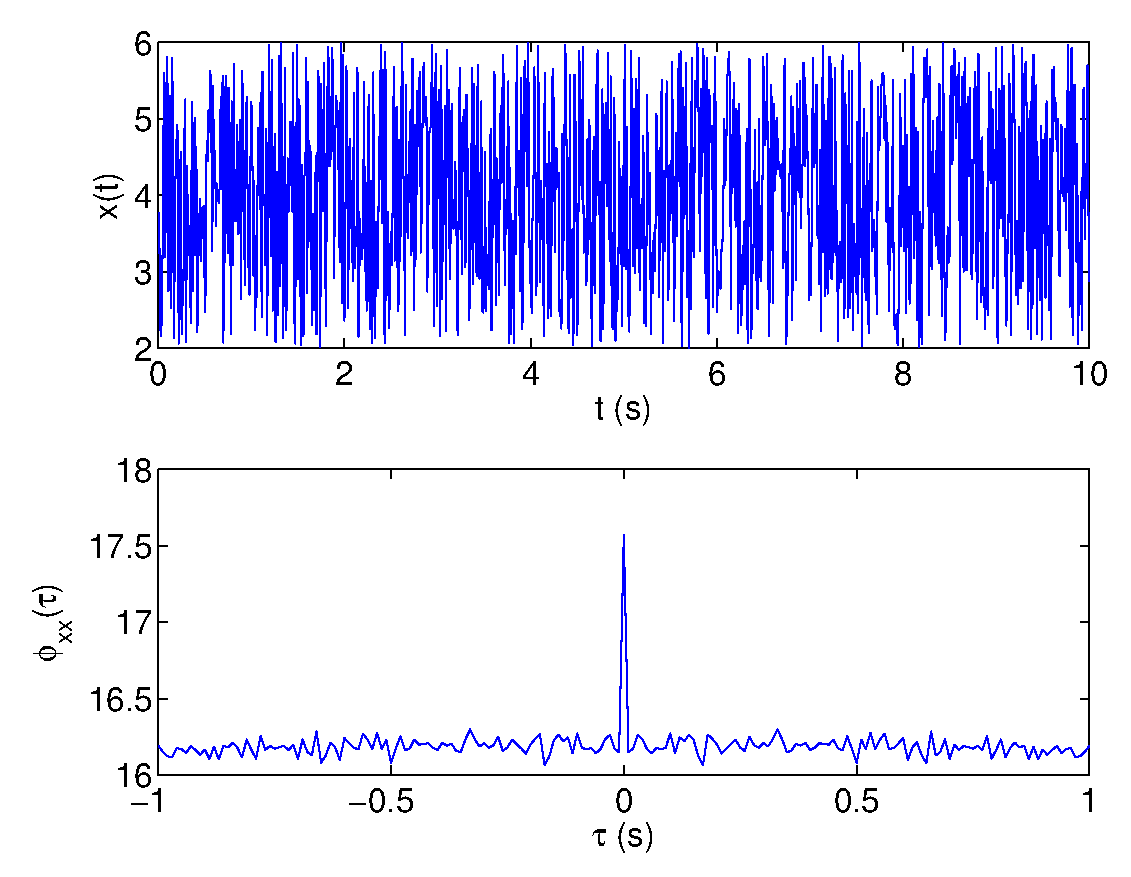
\includegraphics[width=3.2cm]{./Figures/Auto2.eps}

\scriptsize
\color{gray}
$\phi_{XX}(0)\!=\!\Psi_X\!=\!\frac{b^2+a^2+ab}{3}\!=\!17.3$

$\phi_{XX}(\infty) \rightarrow \mu^2_X=\left(\frac{b+a}{2}\right )^2=16$}

\end{column}
\end{columns}


%%%%%%%%%%%%%%%%%%%%%%%%%%%%%%%%%%%%%%%%%%
\vspace{0.3cm}

\visible<3->{
\begin{columns}[c]
\hspace{-0.5cm}\begin{column}{6cm}

\color{olivegreen}Ej3: Sistema continuo determinista con $x(t)=sen(2\pi F t)$ con $F=10$ Hz.

\color{black}

\vspace{0.1cm}

Lo discretizamos con periodo $T_s=0.01$


\vspace{-0.3cm}

\lstinputlisting{./Matlab/Auto3.m}

\end{column}
\begin{column}{4cm}
\visible<4->{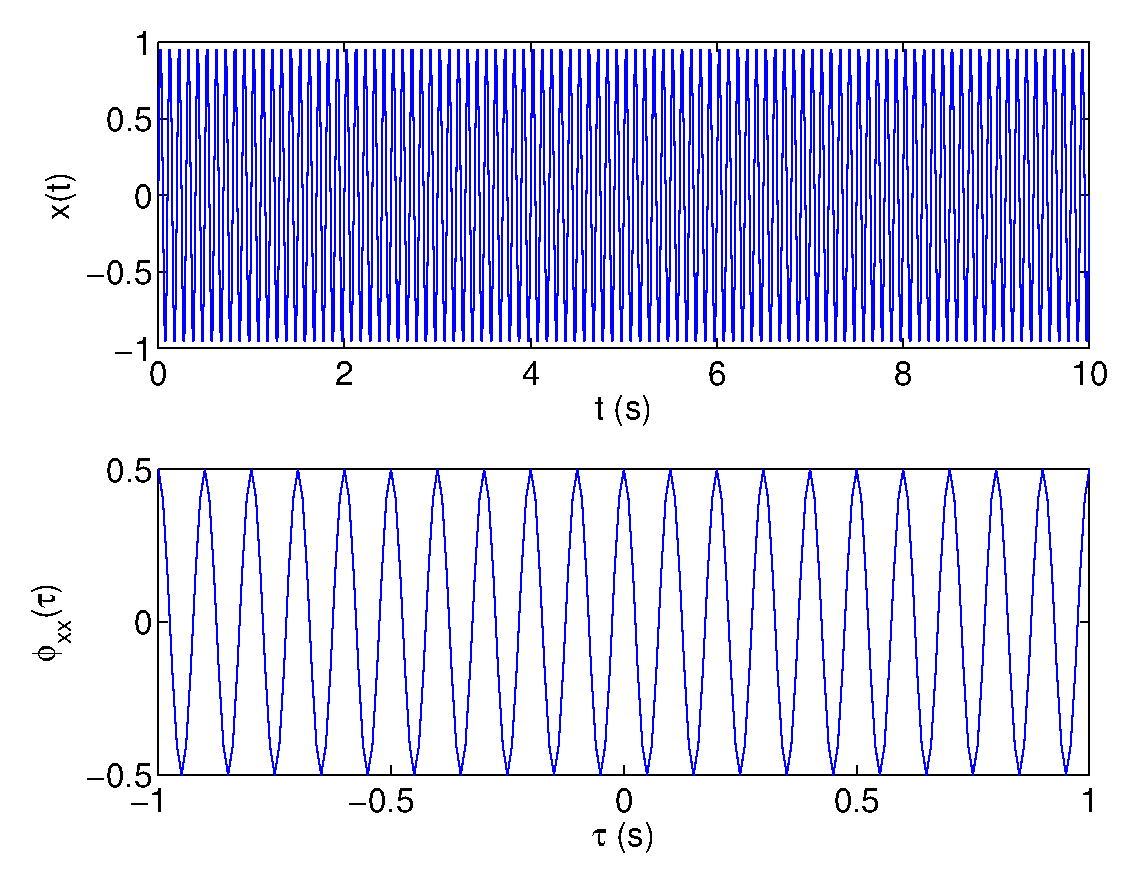
\includegraphics[width=4cm]{./Figures/Auto3.eps}}




\end{column}
\end{columns}}

\end{frame}


%%%%%%%%%%%%%%%%%%%%%%%%%%%%%%%%%%%%%%%%%%%%%%%%

\begin{frame}
\frametitle{Señales aleatorias estacionarias: Propiedades IV}


\footnotesize
\begin{itemize}

\item Relaciones con la correlación cruzada:


\begin{itemize}

\footnotesize

\item No tiene necesariamente un máximo en $\tau=0$

\vspace{0.1cm}

\item $\phi_{XY}(\tau)=\phi_{YX}(-\tau)$

\vspace{0.1cm}

\item  $|\phi_{XY}(\tau)|^2 \le \phi_{XX}(0) \phi_{YY}(0)$

\vspace{0.1cm}

\item  $|\phi_{XY}(\tau)| \le \frac{1}{2} [\phi_{XX}(0) +\phi_{YY}(0)]$

\vspace{0.1cm}

\item  Si las variables son independientes $\phi_{XY}(0)=\mu_X \mu_Y$.

\end{itemize}


\item Utilidades adicionales de la función de correlación cruzada:

\begin{itemize}

\footnotesize

\item Determinar retardos entre señales: esto se debe a que en la zona en la que se superpongan la señal original y la señal retardada aparece un máximo en la señal de correlación cruzada. A veces el pico no es lo suficientemente significativo para para poder determinar el retardo.

\item Determinación de caminos de transmisión con diferentes retardos.

\item Recuperar señales con ruido (podemos calcular la correlación de la señal original sin ruido con la que viene con ruido y determinar los picos donde se superponen).

\end{itemize}

\end{itemize}
\end{frame}

%%%%%%%%%%%%%%%%%%%%%%%%%%%%%%%%%%%%%%%%
\begin{frame}
\frametitle{Señales aleatorias estacionarias: Propiedades V}

\footnotesize


\color{olivegreen}Ejemplos de aplicación de correlación cruzada de señales.

%%%%%%%%%%%%%%%%%%%%%%%%

\vspace{0.2cm}

\begin{columns}[T]
\hspace{-0.3cm}\begin{column}{6cm}

\color{olivegreen}Ej1: Calcular el desfase de las señales $x(t)=sinc(t-2)$ y $y(t)=sinc(t-3)$

\color{black}

\vspace{0.1cm}

Lo discretizamos con periodo $T_s=0.01$

\vspace{-0.4cm}

\lstinputlisting{./Matlab/Corr1.m}

\end{column}
\begin{column}{4cm}
\visible<2->{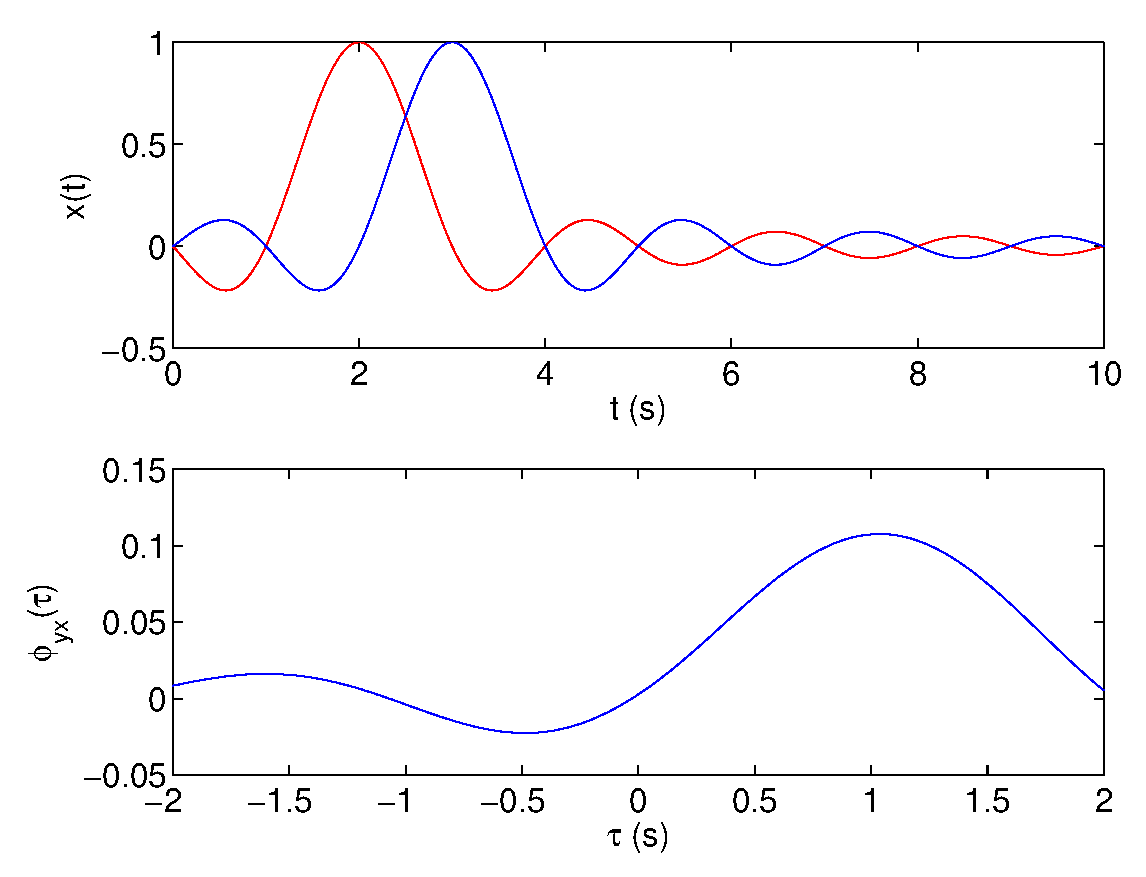
\includegraphics[width=3.2cm]{./Figures/CrossCorr1.eps}

\scriptsize
\color{gray}
Máximo en $\tau=1$, tiempo que está retardada la señal.
}



\end{column}
\end{columns}
\visible<3->{

\vspace{0.2cm}

\begin{columns}[T]
\hspace{-0.35cm}\begin{column}{6cm}

\color{olivegreen}Ej2: Localizar la señal $x(t)=sinc(t-2)$ en $y(t)=sinc(t-3)+u(t)$ con $u(t)\sim \mathcal{N}_U(u,0,4)$

\color{black}

\vspace{0.1cm}

Lo discretizamos con periodo $T_s=0.01$

\vspace{-0.4cm}

\lstinputlisting{./Matlab/Corr2.m}

\end{column}
\begin{column}{4cm}
\visible<4->{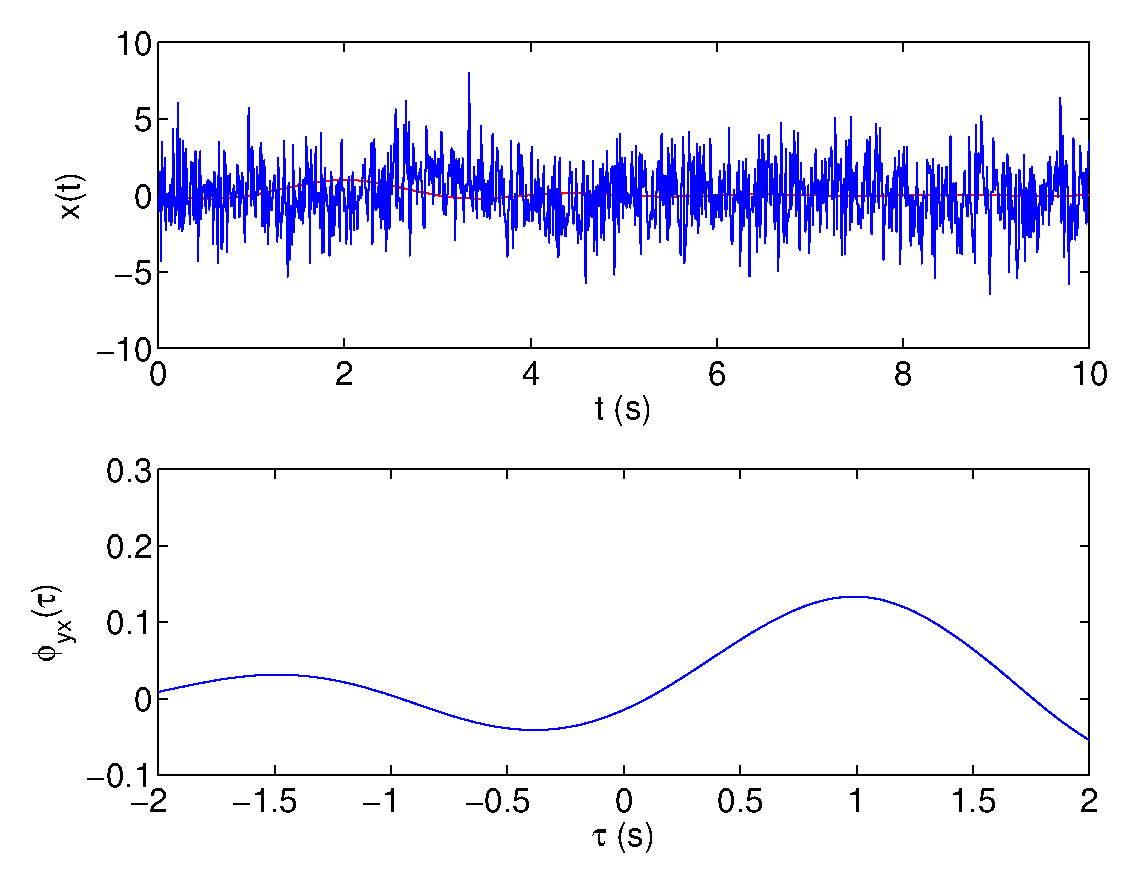
\includegraphics[width=3.2cm]{./Figures/CrossCorr2.eps}

\scriptsize
\color{gray}
Máximo en $\tau=1$,  tiempo que está retardada la señal determinista buscada
}


\end{column}
\end{columns}
}


\end{frame}

 %%%%%%%%%%%%%%Empieza la presentacion%%%%%%%%%%%%%%%%%%%%%%%%%%%%%%%%%%
 

%%%%%%%%%%%%%%%%%%%%%%%%%%%%%%%%%%%%%%%%%%%%%%%%

\begin{frame}
\frametitle{Potencia de una señal aleatoria}
\vspace{-0.2cm}
\footnotesize
\begin{itemize}
\item La potencia de una señal aleatoria se define$^1$ como el valor esperado de la potencia de una señal:

$P_X=E(\lim_{N \rightarrow \infty } \frac{1}{2N+1}\sum_{n=-N}^{N} x^2(n))=\lim_{N \rightarrow \infty } \frac{1}{2N+1} \sum_{n=-N}^{N} E(x^2(n))$

\visible<2->{

\item En los casos en los que  $E(x^2(n))$ es una señal aleatoria estacionaria se cumple que:

\begin{itemize}
\footnotesize
\item$P_X=E(x^2(n))$ (sumario de 2N+1 términos iguales hace que se cancele el denominador de la expresión).
\item $P_X=\phi_{XX}(0)=\sigma^2_X+\mu_x^2$.
\end{itemize}}


\visible<3->{
\item Por lo tanto, en el caso de las señales aleatorias estacionarias, la potencia de la señal se encuentra relacionada con la autocorrelación en el instante inicial$^2$. 
}

\end{itemize}


\rule{11cm}{0.04ex}
\scriptsize
$^1$Vamos a utilizar las definiciones sobre señales discretas en esta caso. Equivalentemente, se podría utilizar la definición sobre continuas, cambiando el sumatorio por la integral.

\vspace{0.1cm}
\visible<3->{
$^2$Este hecho hace que la autocorrelación se entienda como una potencia generalizada variable con $\tau$.
}

\end{frame}


%%%%%%%%%%%%%%%%%%%%%%%%%%%%%%%%%%%%%%%%%%%%%%%%

\begin{frame}
\frametitle{Transformada de Fourier de señales aleatorias}
\vspace{-0.2cm}
\footnotesize
\begin{itemize}
\footnotesize

\item Las transformadas de Fourier representativas (es decir, que mejor caracterizan) a las señales aleatorias no son la transformada de una muestra/secuencia de la señal, si no  las de las señales de autocorrelacion y correlación cruzada.
\visible<2->{
\item \alert{La densidad espectral de potencia}$^1$  es la transformada de Fourier de la señal de autocorrelación:

\begin{itemize}

\footnotesize

\item Continuo: $\Phi_{XX}(jw)=\int_{-\infty}^{\infty} \phi_{XX}(\tau)e^{-jw\tau}d\tau$

\vspace{0.1cm}

\item Discreto: $\Phi_{XX}(e^{jw})=\sum_{l=-\infty}^{\infty} \phi_{XX}(l)e^{-jwl}$

\vspace{0.1cm}

\item El espectro de potencia permite clasificar las señales aleatorias: ruido blanco, señal aleatoria de banda ancha, señal aleatoria de banda estrecha. 
\end{itemize}

}

\visible<3->{
\item \alert{La densidad espectral cruzada} es la transformada de Fourier de la señal de correlación cruzada:

\begin{itemize}

\footnotesize

\item Continuo: $\Phi_{XY}(jw)=\int_{-\infty}^{\infty} \phi_{XY}(\tau)e^{-jw\tau}d\tau$

\vspace{0.1cm}

\item Discreto: $\Phi_{XY}(e^{jw})=\sum_{l=-\infty}^{\infty} \phi_{XY}(l)e^{-jwl}$

\vspace{0.1cm}

\end{itemize}


}


\end{itemize}


\rule{11cm}{0.04ex}
\scriptsize
También se denomina espectro de densidad de potencia o simplemente espectro de potencia.

\end{frame}


%%%%%%%%%%%%%%%%%%%%%%%%%%%%%%%%%%%%%%%%%%%%%%%%

\begin{frame}
\frametitle{Clasificación de las señales aleatorias}
\vspace{-0.2cm}
\footnotesize
\begin{itemize}
\footnotesize
\item Señal de ruido blanco: aquella cuyo espectro en potencia toma valor constante
\begin{itemize}
\footnotesize
\scriptsize
\item Continuo: $\Phi_{XX}(jw)=a$   $\rightarrow \phi_{XX}(\tau)=a\delta(\tau)$.

\vspace{0.1cm}

 No es físicamente realizable, ya que tendría que ser una señal de potencia infinita (ya que $P_X=\phi_{XX}(\tau=0)=\infty$). 
 
 \vspace{0.1cm}
 
 \item Discreto: $\Phi_{XX}(e^{jw})=a $  $\rightarrow \phi_{XX}(l)=a \delta(l)$.
 
 
\end{itemize}

\item Señal con bias constante: aquella cuya autocorrelación toma un valor constante:
\begin{itemize}
\footnotesize
\scriptsize
\item Continuo: $\Phi_{XX}(jw)=\mu^2_X \delta(w)$   $\leftarrow \phi_{XX}(\tau)=\mu^2_X$.

\vspace{0.1cm}

 \item Discreto: $\Phi_{XX}(e^{jw})=\mu^2_X \delta(w)$   $\leftarrow \phi_{XX}(l)=\mu^2_X$.

 
 \vspace{0.1cm}
 
 
\end{itemize}


 \item Una combinación de las dos anteriores
 
 \item Señal aleatoria con espectro en potencia paso baja: es la que su espectro en potencia tiene la forma de un filtro paso bajo ideal.
 
 \item Señal aleatoria con espectro en potencia paso banda: es la que su espectro en potencia tiene la forma de un filtro paso banda ideal.

\item Señal aleatoria de banda estrecha: aquella cuyo espectro en frecuencia tiene una banda en frecuencias estrecha

\item Señal aleatoria de banda ancha: aquella cuyo espectro en frecuencia tiene una banda en frecuencia ancha.


\end{itemize}
\end{frame}


%%%%%%%%%%%%%%%%%%%%%%%%%%%%%%%%%%%%%%%%%%%%%%%%

\begin{frame}
\frametitle{Procesamiento de señales aleatorias I}
\vspace{-0.2cm}
\footnotesize
\begin{itemize}
\item Las señales aleatorias, como señales que son, se pueden procesar con todos los sistemas lineales y filtros ideales con los que hemos trabajado a lo largo de la asignatura.
\item Pero debido a su aleatoreidad, para caracterizar su comportamiento correctamente necesitamos estudiar que le sucede a la función de probabilidad o a los estadísticos de la señal aleatoria filtrada. 
\item Esto se pude hacer determinando que le sucede a la media, al valor cuadrático medio, autocorrelación, etc ... de la señal de salida del filtro $H(s)$ o $H(z)$ a partir de los valores de los estadísticos correspondientes de la señal de entrada.
\item El análisis se puede realizar tanto en continuo como en discreto. En nuestro caso, realizaremos en discreto el análisis restante del tema.
\item Y en todo momento vamos a suponer que los sistemas lineales/filtros son deterministas, y que por lo tanto, la aleatoreidad del proceso se encuentra únicamente asociado a la aleatoreidad de la señal. 
\item Además, también supondremos que las señales aleatorias son estacionarias (en el sentido amplio).


\end{itemize}
\end{frame}


%%%%%%%%%%%%%%%%%%%%%%%%%%%%%%%%%%%%%%%%%%%%%%%%%


\begin{frame}
\frametitle{Procesamiento de señales aleatorias II}
\vspace{-0.2cm}
\footnotesize
\begin{itemize}
\item La respuesta de un sistema determinista a cualquier entrada se puede calcular a través de la función de convolución: $y(n)=(h*x)(n)=\sum_{k=-\infty}^{\infty} h(k)x(n-k)$ 

\visible<2->{
\item El valor medio de la señal de salida:
\alert{$\mu_Y=H(e^{j0})\mu_X$}

{\scriptsize

\color{gray}
Se calcula aprovechando las propiedades de la linealidad del sistema

$\mu_Y=E(y(n))=E(\sum_{k=-\infty}^{\infty} h(k)x(n-k))=\sum_{k=-\infty}^{\infty} h(k)E(x(n-k))=$

\hspace{0.8cm}$=\mu_X \sum_{k=-\infty}^{\infty} h(k)=H(e^{j0})\mu_X$
\color{black}}}

\visible<3->{

\item La señal de autocorrelación (productos aparecen en el dominio de la frecuencia): \alert{$\Phi_{YY}(e^{jw})=|H(e^{jw})H(e^{-jw})|\Phi_{XX}(e^{jw})$}

{\scriptsize
\color{gray}

$\phi_{YY}(l)\!=\!E(y(n\!+\!l)y(n))\!=\!E\!\!\left (\left ( \sum_{i=-\infty}^{\infty} h(i)x(n\!+\!l\!-\!i) \right )\!\! \left ( \sum_{k=-\infty}^{\infty} h(k)x(n\!-\!k) \right )\right )=$

\hspace{0.9cm}$=\sum_{i=-\infty}^{\infty} h(i) \sum_{k=-\infty}^{\infty} h(k) E(x(n\!+\!l\!-\!i)x(n\!-\!k))=^1$

\vspace{0.1cm}

\hspace{0.9cm}$=\sum_{i=-\infty}^{\infty} h(i) \sum_{k=-\infty}^{\infty} h(k) \psi_{XX}(l+k-i)=^2$

\vspace{0.1cm}

\hspace{0.9cm}$=\sum_{m=-\infty}^{\infty} \psi_{XX}(l-m) \sum_{k=-\infty}^{\infty} h(k) h(m+k) =(\psi_{XX}*(h(k)*h(-k))(l)$

\vspace{0.1cm}

En el dominio de la transformada las operaciones son más sencillas: dos convoluciones sucesivas se convierten en dos productos.



$\phi_{YY}(e^{jw})=|H(e^{jw})H(e^{-jw})|\Phi_{XX}(e^{jw})$

}}

\end{itemize}

\vspace{-0.2cm}

\rule{11cm}{0.04ex}

\visible<3->{
\color{gray}
\scriptsize
$^1$Como son señales estacionarias el valor esperado solo depende de la diferencia de los indices: $E(x(n\!+\!l\!-\!i)x(n\!-\!k))=\psi_{XX}(l+k-i)$

$^2$Cambio de variable $m=i-k$
}


\end{frame}


\begin{frame}
\frametitle{Procesamiento de señales aleatorias III}
\vspace{-0.2cm}
\footnotesize
\begin{itemize}
\item La señal de autocorrelacion: \alert{$\Phi_{YY}(e^{jw})=|H(e^{jw})H(e^{-jw})|\Phi_{XX}(e^{jw})$}
\begin{itemize}
\footnotesize
\item Utilidad: La expresión es especialmente útil para obtener el espectro en frecuencia de un sistema lineal con una función de transferencia desconocida:

\visible<2->{
\begin{itemize}
\footnotesize
\item  Para eso basta con excitar el sistema con una señal aleatoria estacionaria $x(n)$ de espectro en potencia conocido y observar el espectro en potencia de la señal de salida.
 
\item El cociente de ambos espectros nos da el cuadrado del módulo del espectro del sistema lineal.  
\end{itemize}}
\end{itemize}

\visible<3->{
\item La señal de correlación cruzada: \alert{$\Phi_{XY}(e^{jw})=H(e^{jw})\Phi_{XX}(e^{jw})$}

\begin{itemize}
\footnotesize
\item La demostración es análoga a la anterior, calculando la correlación entre la señal de salida (que pasa una vez por el sistema) y la señal de entrada (que no pasa por el filtro). 
\item En este caso, la expresión nos relaciona el espectro de potencia de la señal de entrada con la densidad espectral cruzada de la entrada y la salida. 
\item Utilidad similar a la del caso anterior, pero ahora podemos obtener la respuesta en frecuencia completa.
\end{itemize}}


\end{itemize}
\end{frame}


\end{document}
